\chapter{Árvores Binárias Aleatórias de Busca}
\chaplabel{rbs}

Neste capítulo, apresentamos uma estrutura de árvore binária de busca que usa a aleatoriedade para conseguir $O(\log #n#)$ de tempo esperado para todas as operações.

\section{Árvores Binárias Aleatórias de Busca}
\seclabel{rbst}

Considere as duas árvores binárias de busca mostradas na \figref{rbs-lvc}, cada uma das quais possui $#n#=15$ nós.  A árvore da esquerda é uma lista e a outra é uma árvore binária de busca perfeitamente balanceada. A árvore da esquerda possui uma altura de $#n#-1=14$ e aquela à direita possui uma altura de três.

\begin{figure}
  \begin{center}
    \begin{tabular}{cc}
      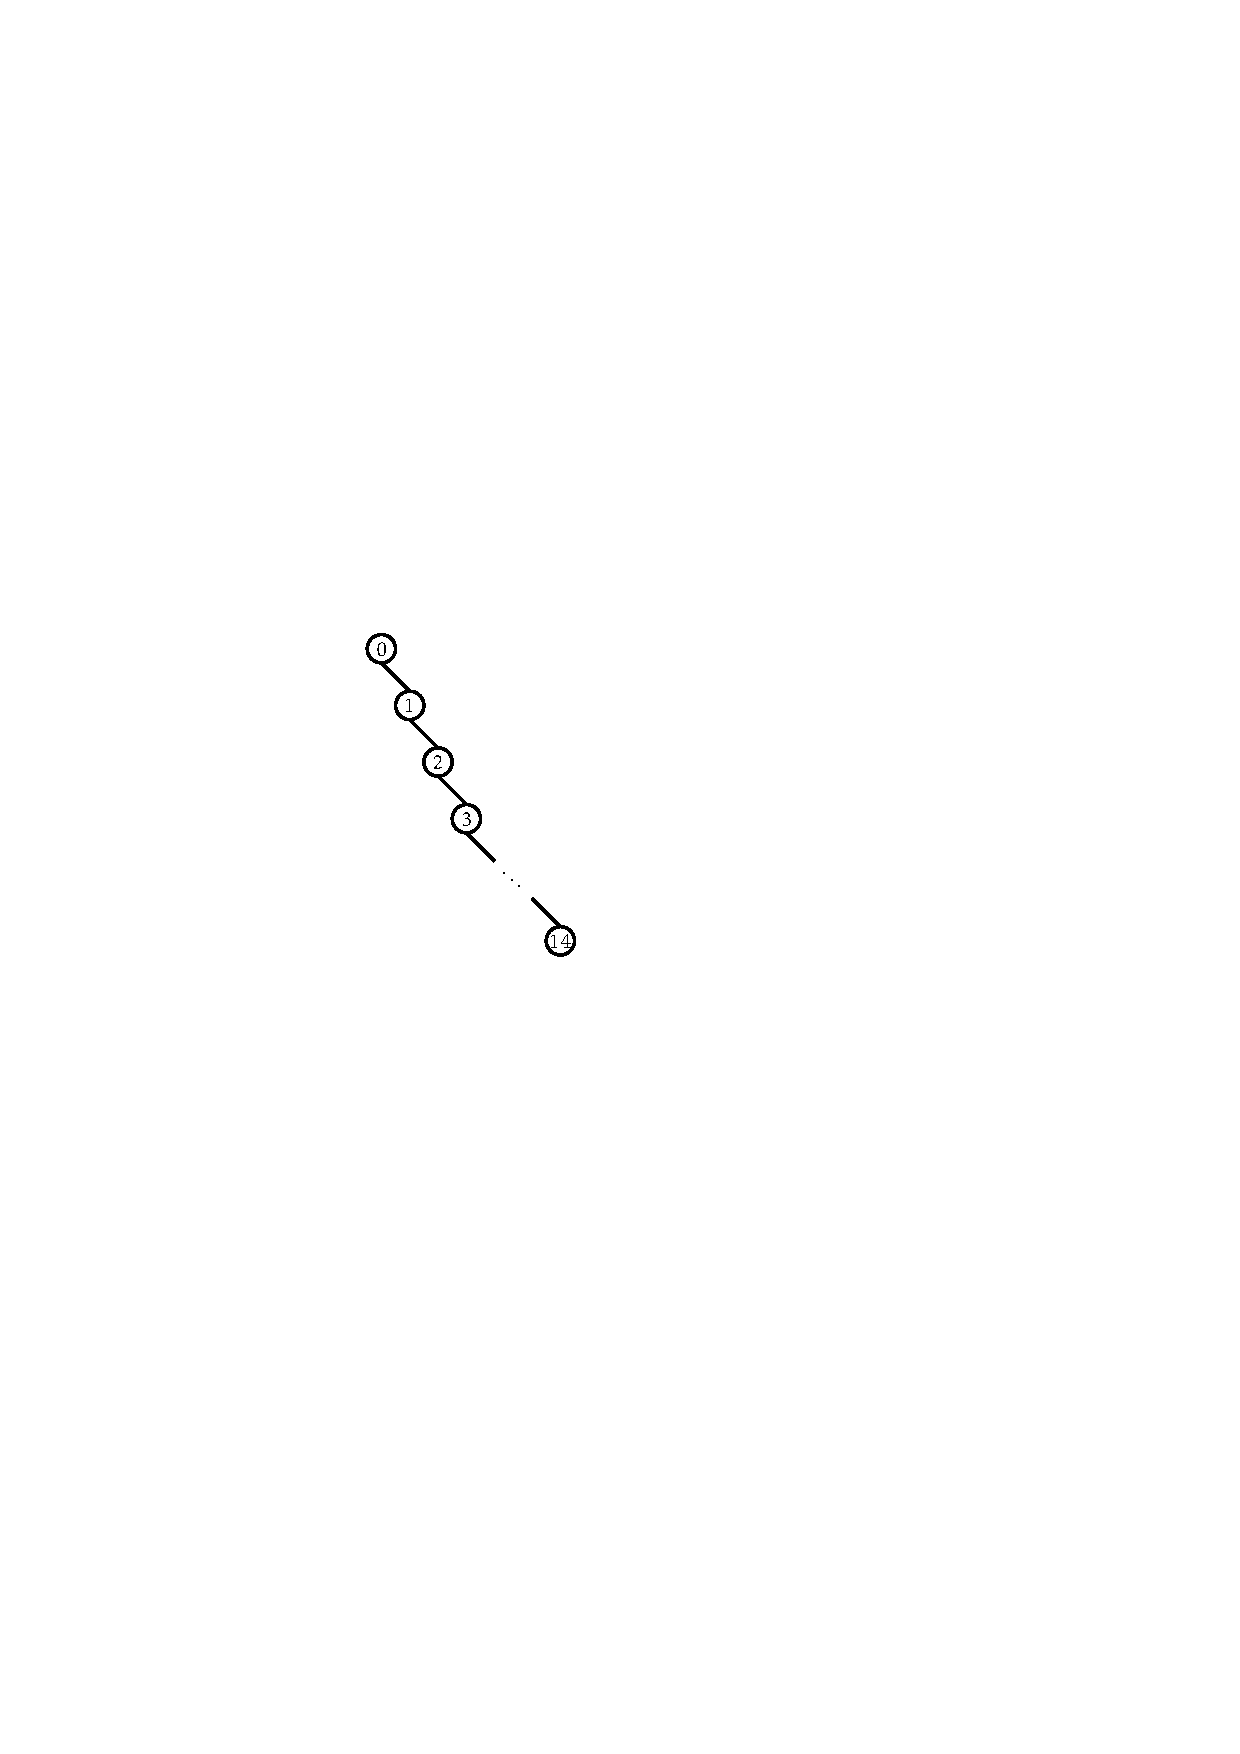
\includegraphics[scale=0.90909,scale=0.95]{figs/bst-path} &
      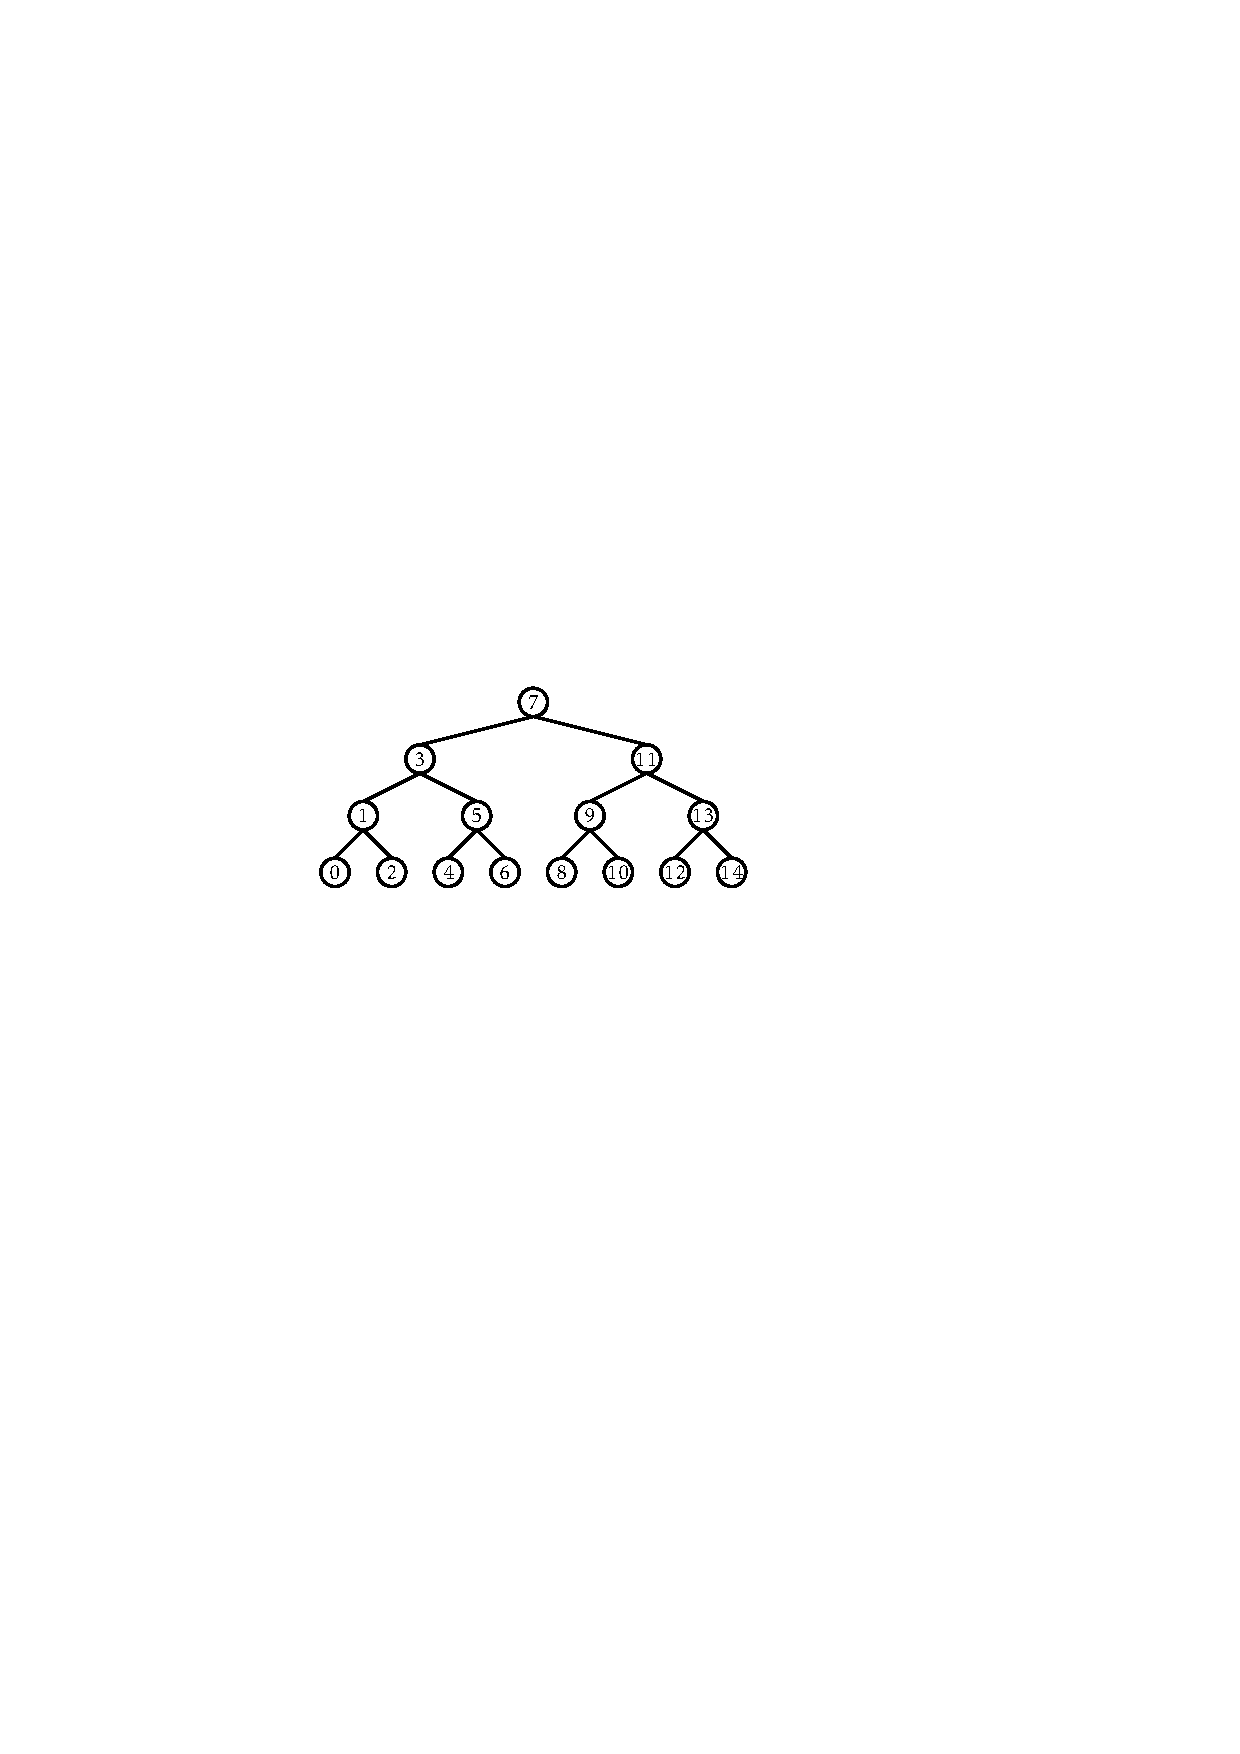
\includegraphics[scale=0.90909,scale=0.95]{figs/bst-balanced}
    \end{tabular}
  \end{center}
  \caption{Duas árvores binárias de busca com inteiros $0,\ldots,14$.}
  \figlabel{rbs-lvc}
\end{figure}

Imagine como essas duas árvores poderiam ser construídas.  A árvore da esquerda ocorre se começamos com uma #ArvoreBinariaDeBusca# vazia e acrescentamos a sequência

\[
    \langle 0,1,2,3,4,5,6,7,8,9,10,11,12,13,14 \rangle \enspace .
\]
Nenhuma outra sequência de adições vai criar esta árvore (como você pode provar por indução em #n#). Por outro lado, a árvore da direita pode ser criada pela sequência
\[
    \langle 7,3,11,1,5,9,13,0,2,4,6,8,10,12,14 \rangle  \enspace .
\]
Outras sequências funcionam bem, incluindo
\[
    \langle 7,3,1,5,0,2,4,6,11,9,13,8,10,12,14 \rangle  \enspace ,
\]
e
\[
    \langle 7,3,1,11,5,0,2,4,6,9,13,8,10,12,14 \rangle \enspace .
\]
De fato, existem $21,964,800$ sequências que geram a árvore da direita e somente uma que gera a árvore da esquerda.

O exemplo acima nos dá uma evidência factual que, se escolhemos uma permutação aleatória de $0,\ldots,14$, e inserimos em uma árvore binária, é mais provável obtermos uma árvore balanceada (a árvore da direita de \figref{rbs-lvc}) que obtermos uma árvore totalmente desbalanceada (aquela do lado esquerdo de \figref{rbs-lvc}).

Podemos formalizar esta noção estudando as árvores binárias aleatórias de busca.
Uma \emph{árvore binária aleatória de busca}
\index{árvore binária aleatória de busca}%
\index{árvore binária de busca!aleatória}%
de tamanho #n# é obtida do seguinte modo:  
Considere uma permutação aleatória, $#x#_0,\ldots,#x#_{#n#-1}$,
de inteiros $0,\ldots,#n#-1$ e insira seus elementos, um a um,
em uma #ArvoreBinariaDeBusca#.  Por \emph{permutação aleatória}
\index{permutação!aleatória}%
\index{permutação aleatória}%
queremos dizer
que cada possível $#n#!$ permutação (ordenação) de $0,\ldots,#n#-1$
é igualmente provável, assim como que a probabilidade de obter qualquer permutação particular é $1/#n#!$.

Note que os valores $0,\ldots,#n#-1$ poderiam ser substituídos por qualquer conjunto ordenado de #n# elementos sem mudar qualquer uma das propriedades da 
árvore binária aleatória de busca.  O  elemento $#x#\in\{0,\ldots,#n#-1\}$ significa
apenas o elemento de ordem #x# de um conjunto ordenado de tamanho #n#.

Antes de apresentarmos nosso resultado principal sobre árvores binárias aleatórias de busca,
devemos tomar um tempo para uma curta digressão para discutir um tipo de número
que aparece frequentemente quando estudamos estruturas aleatórias. Para um 
inteiro não negativo, $k$, o $k$-ésimo \emph{número harmônico},
\index{número harmônico}%
\index{H@$H_k$ (número harmônico)}%
identificado por
$H_k$, é definido como
\[
  H_k = 1 + 1/2 + 1/3 + \cdots + 1/k \enspace .
\] 
O número harmônico $H_k$ não tem uma forma analítica simples, porém ele
é ligado de forma muito estreita ao logaritmo natural de $k$.  Particularmente,
\[
  \ln k < H_k \le \ln k + 1  \enspace .
\]
\newcommand{\hint}{\int_1^k\! (1/x)\, \mathrm{d}x}%
Leitores que estudaram cálculo podem notar que isto ocorre porque
a integral $\hint = \ln k$.  Percebendo que uma integral pode ser
interpretada como a área entre uma curva e o eixo $x$, o valor de
$H_k$ pode ter como limite inferior a integral $\hint$ e como limite superior
$1+ \hint$.  (Veja \figref{harmonic-integral} para uma explicação gráfica.)

\begin{figure}
  \begin{center}
    \begin{tabular}{cc}
      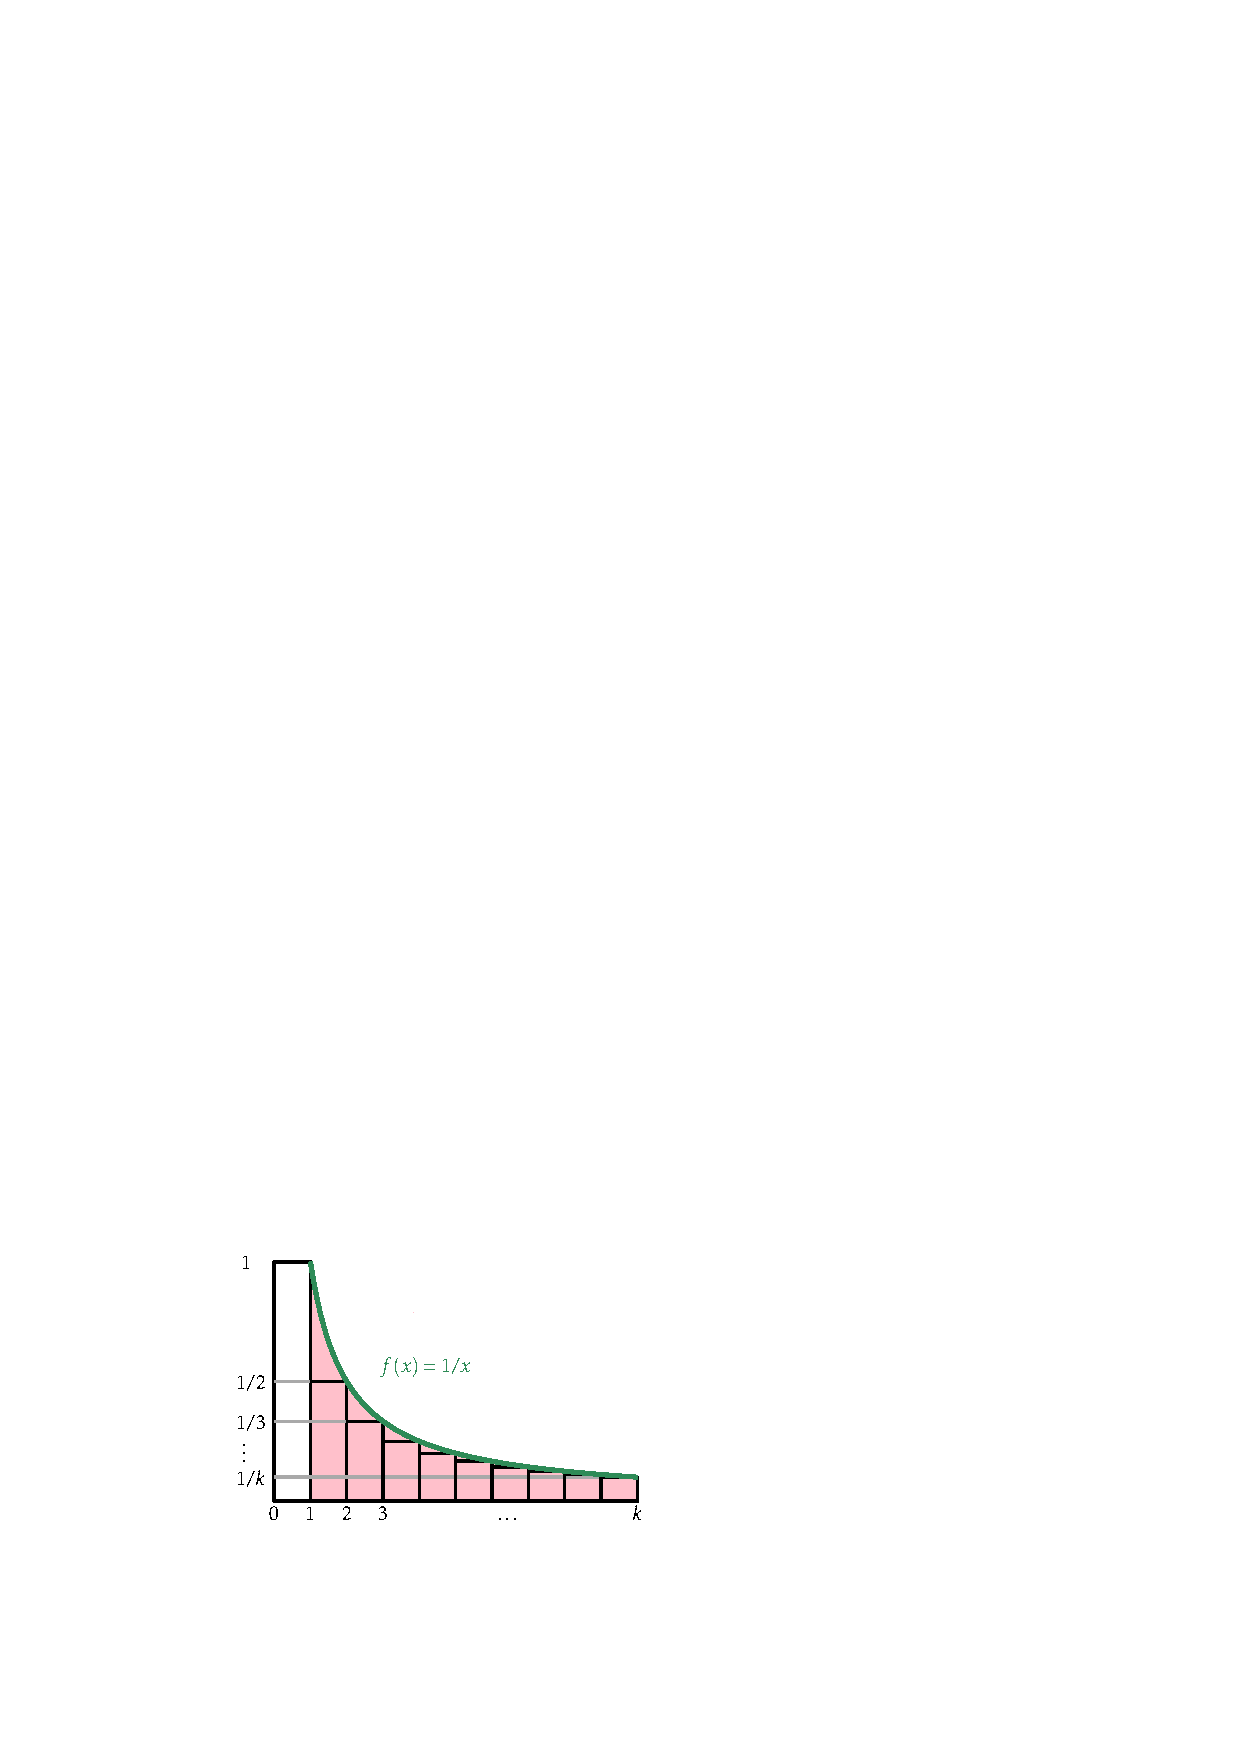
\includegraphics[width=\HalfScaleIfNeeded]{figs/harmonic-2} 
        & 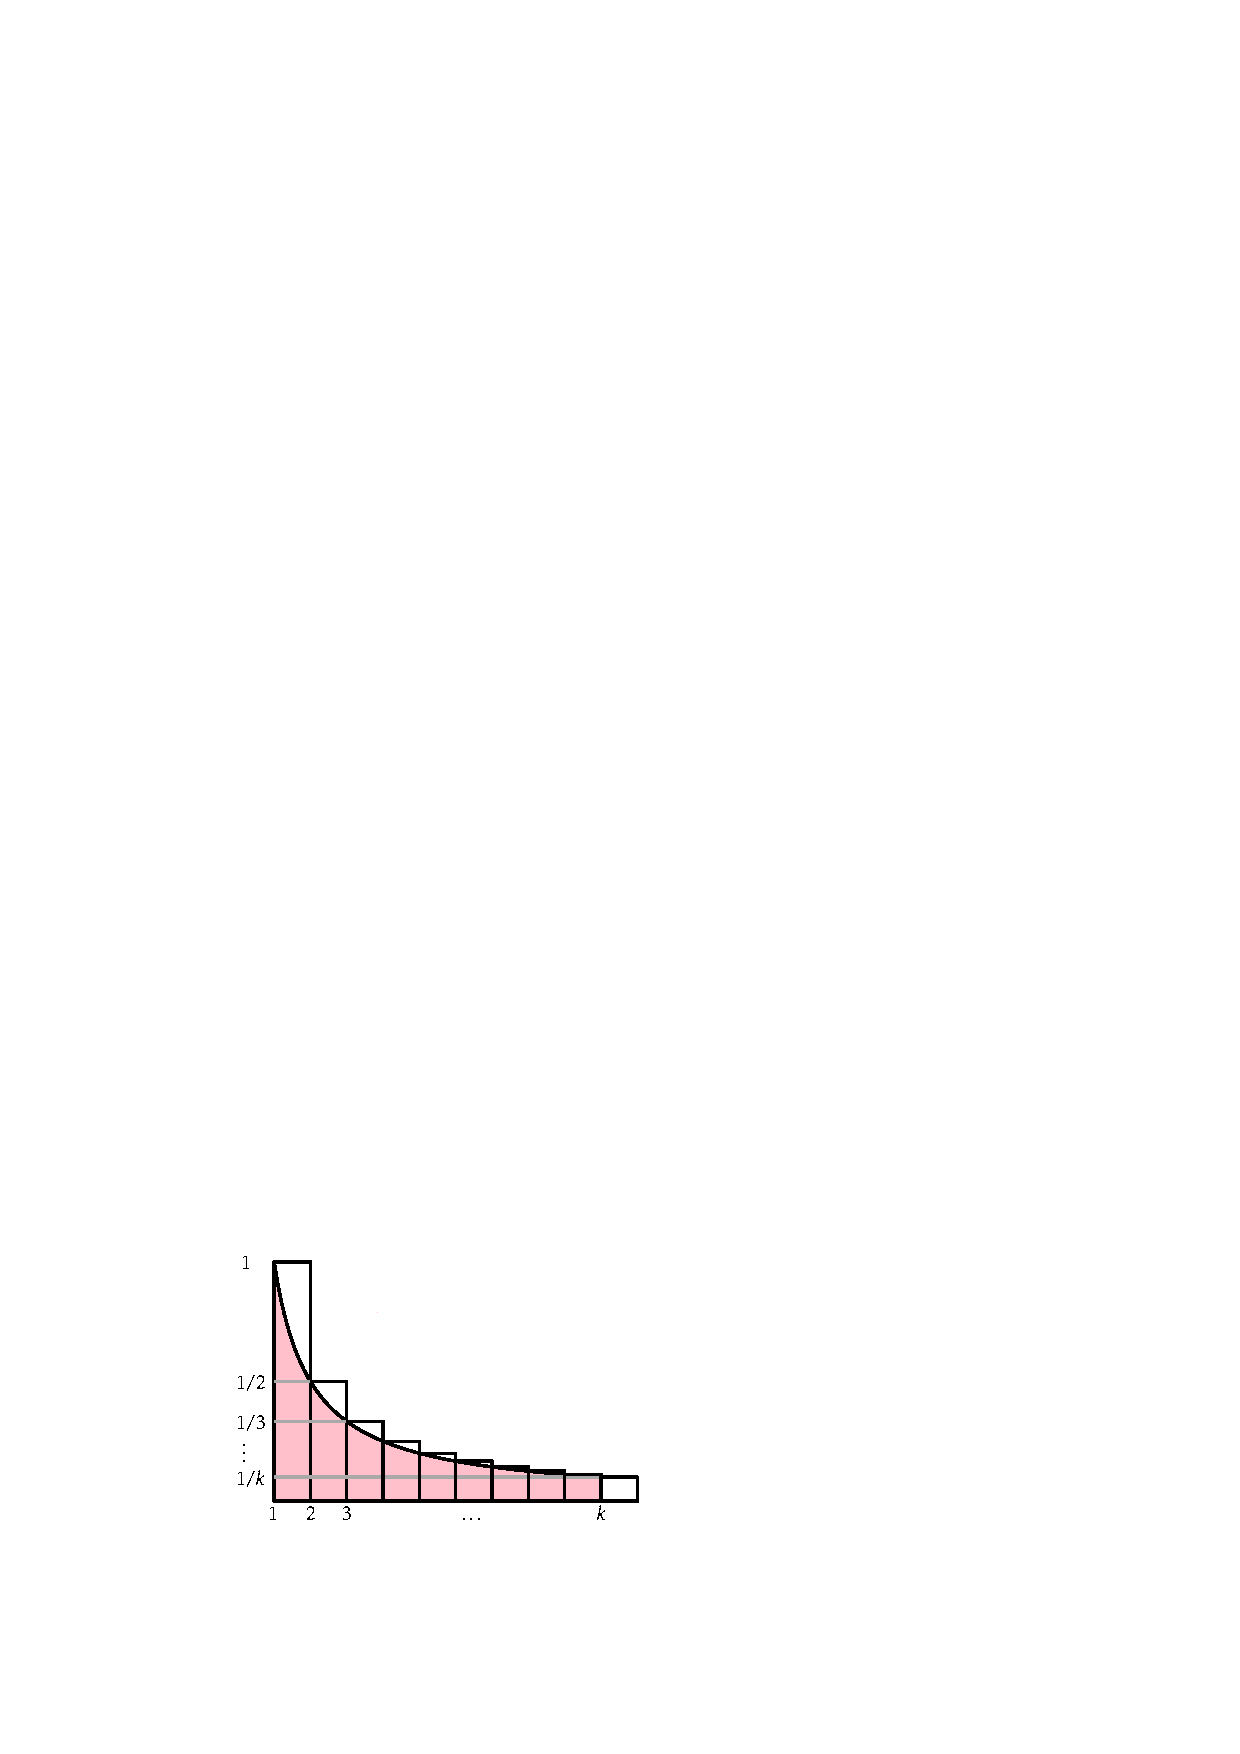
\includegraphics[width=\HalfScaleIfNeeded]{figs/harmonic-3}
    \end{tabular}
  \end{center}
  \caption{O $k$ésimo número harmônico $H_k=\sum_{i=1}^k 1/i$ tem limite superior e inferior dados por duas integrais. O valor dessas integrais é dado pela área da região sombreada, enquanto o valor de $H_k$ é dado pela área dos retângulos.}
  \figlabel{harmonic-integral}
\end{figure}


\begin{lem}\lemlabel{rbs}
  Em uma árvore binária aleatória de busca de tamanho #n#, as seguintes declarações são verdadeiras:
  \begin{enumerate}
    \item Para qualquer $#x#\in\{0,\ldots,#n#-1\}$, o comprimento esperado do 
    caminho de busca para #x# é $H_{#x#+1} + H_{#n#-#x#} - O(1)$.\footnote{As 
    expressões $#x#+1$ e $#n#-#x#$ podem ser interpretadas respectivamente
    como o número de elementos na árvore menores que ou iguais a #x#
    e o número de elementos na árvore maiores que ou iguais a #x#.}
    \item Para qualquer $#x#\in(-1,n)\setminus\{0,\ldots,#n#-1\}$, o
    comprimento esperado do caminho de busca para #x# é $H_{\lceil#x#\rceil}
    + H_{#n#-\lceil#x#\rceil}$.
  \end{enumerate}
\end{lem}

Vamos provar \lemref{rbs} na próxima seção.  Por agora, considere o que
as duas partes de \lemref{rbs} nos dizem.  A primeira parte nos diz que se
procuramos por um elemento em uma árvore de tamanho #n#, então o comprimento esperado
do caminho de busca é no máximo $2\ln n + O(1)$.  A segunda parte nos diz
a mesma coisa sobre a busca de um valor que não esteja armazenado na árvore.
Quando comparamos a duas partes do lema, vemos que é somente ligeiramente
mais rápido procurar por algo que esteja na árvore do que por algo que 
não esteja.


\subsection{Prova de \lemref{rbs}}

A observação chave necessária para provar o \lemref{rbs} é a seguinte:
O caminho de busca para um valor #x# no intervalo aberto $(-1,#n#)$ em uma
árvore binária aleatória de busca, $T$, contém o nó com a chave $i < #x#$
se, e somente se, na permutação aleatória usada para criar $T$, $i$
apareça antes de qualquer um de $\{i+1,i+2,\ldots,\lfloor#x#\rfloor\}$.

Para ver isso, olhe a \figref{rbst-records} e note que até que
algum valor de $\{i,i+1,\ldots,\lfloor#x#\rfloor\}$ seja inserido, os caminhos
de busca para cada valor no intervalo aberto $(i-1,\lfloor#x#\rfloor+1)$
são idênticos.  (Lembre-se que para dois valores terem
caminhos de busca diferentes, deve existir algum elemento na árvore que
seja comparado diferentemente entre eles.)  Seja $j$ o primeiro elemento em
$\{i,i+1,\ldots,\lfloor#x#\rfloor\}$ a aparecer na permutação aleatória.
Note que $j$ está neste momento e sempre estará no caminho de busca de #x#.
Se $j\neq i$ então o nó $#u#_j$ contendo $j$ é criado antes do
nó $#u#_i$ que contém $i$.  Mais tarde, quando $i$ for inserido, ele será
inserido na subárvore com raiz em $#u#_j#.esquerdo#$, posto que $i<j$.  Por outro lado,
o caminho de busca para #x# nunca passará por esta subárvore porque
ele seguirá para $#u#_j#.direito#$ após visitar $#u#_j$.

\begin{figure}
  \begin{center}
    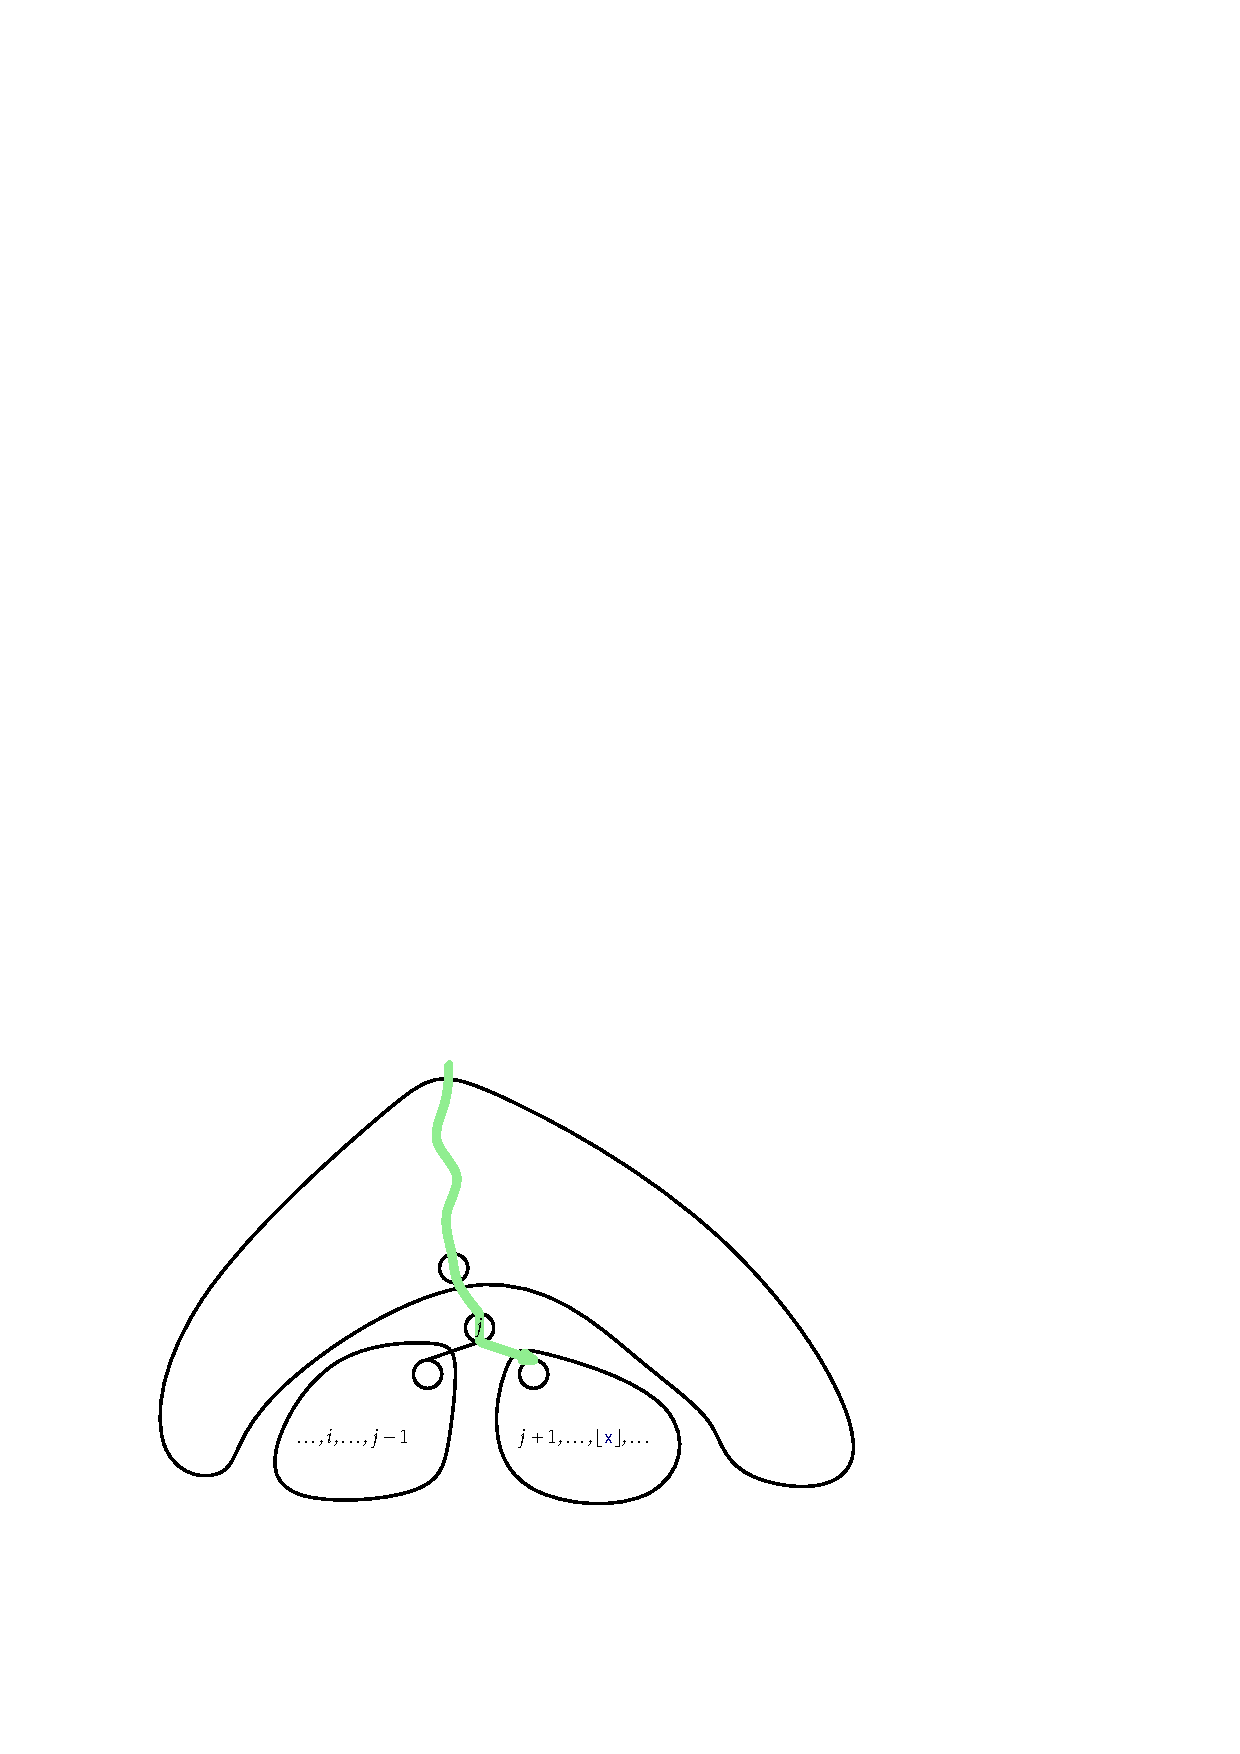
\includegraphics[width=\ScaleIfNeeded]{figs/rbst-records}
  \end{center}
  \caption[O caminho de busca em um árvore binária aleatória de busca]{O valor $i<#x#$ está no caminho de busca para #x# se e somente
   se $i$ é o primeiro elemento entre $\{i,i+1,\ldots,\lfloor#x#\rfloor\}$ inserido na árvore.}
  \figlabel{rbst-records}
\end{figure}

De maneira análoga, para $i>#x#$, $i$ aparece no caminho de busca para #x#
se e somente se $i$ aparece antes de qualquer um de $\{\lceil#x#\rceil,
\lceil#x#\rceil+1,\ldots,i-1\}$ em uma permutação aleatória usada para criar $T$.

Note que, se começamos com uma permutação aleatória de $\{0,\ldots,#n#\}$,
então as subsequências contendo somente $\{i,i+1,\ldots,\lfloor#x#\rfloor\}$
e $\{\lceil#x#\rceil, \lceil#x#\rceil+1,\ldots,i-1\}$ são também permutações
aleatórias de seus respectivos elementos.  Cada elemento, então, nos
subconjuntos $\{i,i+1,\ldots,\lfloor#x#\rfloor\}$ e $\{\lceil#x#\rceil,
\lceil#x#\rceil+1,\ldots,i-1\}$ é igualmente provável de aparecer antes
de qualquer outro no seu subconjunto na permutação aleatória usada para criar $T$.
Assim, temos
\[
  \Pr\{\mbox{$i$ está no caminho de busca para #x#}\}
  = \left\{ \begin{array}{ll}
     1/(\lfloor#x#\rfloor-i+1) & \mbox{if $i < #x#$} \\
     1/(i-\lceil#x#\rceil+1) & \mbox{if $i > #x#$} 
     \end{array}\right . \enspace .
\]

Com esta observação, a prova de \lemref{rbs}
envolve alguns cálculos simples com números harmônicos:

\begin{proof}[Prova de \lemref{rbs}]
Seja $I_i$ a variável aleatória indicadora que é igual a um quando $i$
aparece no caminho de busca para #x# e zero caso contrário.  Então o comprimento
do caminho de busca é dado por
\[
  \sum_{i\in\{0,\ldots,#n#-1\}\setminus\{#x#\}} I_i
\]
deste modo, se $#x#\in\{0,\ldots,#n#-1\}$, o comprimento esperado do caminho de busca
é dado por (veja \figref{rbst-probs}.a)
\begin{align*}
  \E\left[\sum_{i=0}^{#x#-1} I_i + \sum_{i=#x#+1}^{#n#-1} I_i\right]
   & =  \sum_{i=0}^{#x#-1} \E\left[I_i\right]
         + \sum_{i=#x#+1}^{#n#-1} \E\left[I_i\right] \\
   & = \sum_{i=0}^{#x#-1} 1/(\lfloor#x#\rfloor-i+1)
         + \sum_{i=#x#+1}^{#n#-1} 1/(i-\lceil#x#\rceil+1) \\
   & = \sum_{i=0}^{#x#-1} 1/(#x#-i+1)
         + \sum_{i=#x#+1}^{#n#-1} 1/(i-#x#+1) \\
   & = \frac{1}{2}+\frac{1}{3}+\cdots+\frac{1}{#x#+1} \\
   & \quad {} + \frac{1}{2}+\frac{1}{3}+\cdots+\frac{1}{#n#-#x#} \\
   & = H_{#x#+1} + H_{#n#-#x#} - 2  \enspace .
\end{align*}
Os cálculos correspondentes para o valor de busca
$#x#\in(-1,n)\setminus\{0,\ldots,#n#-1\}$ são praticamente idênticos (veja
\figref{rbst-probs}.b).
\end{proof}

\begin{figure}
  \begin{center}
    \begin{tabular}{@{}c@{}}
      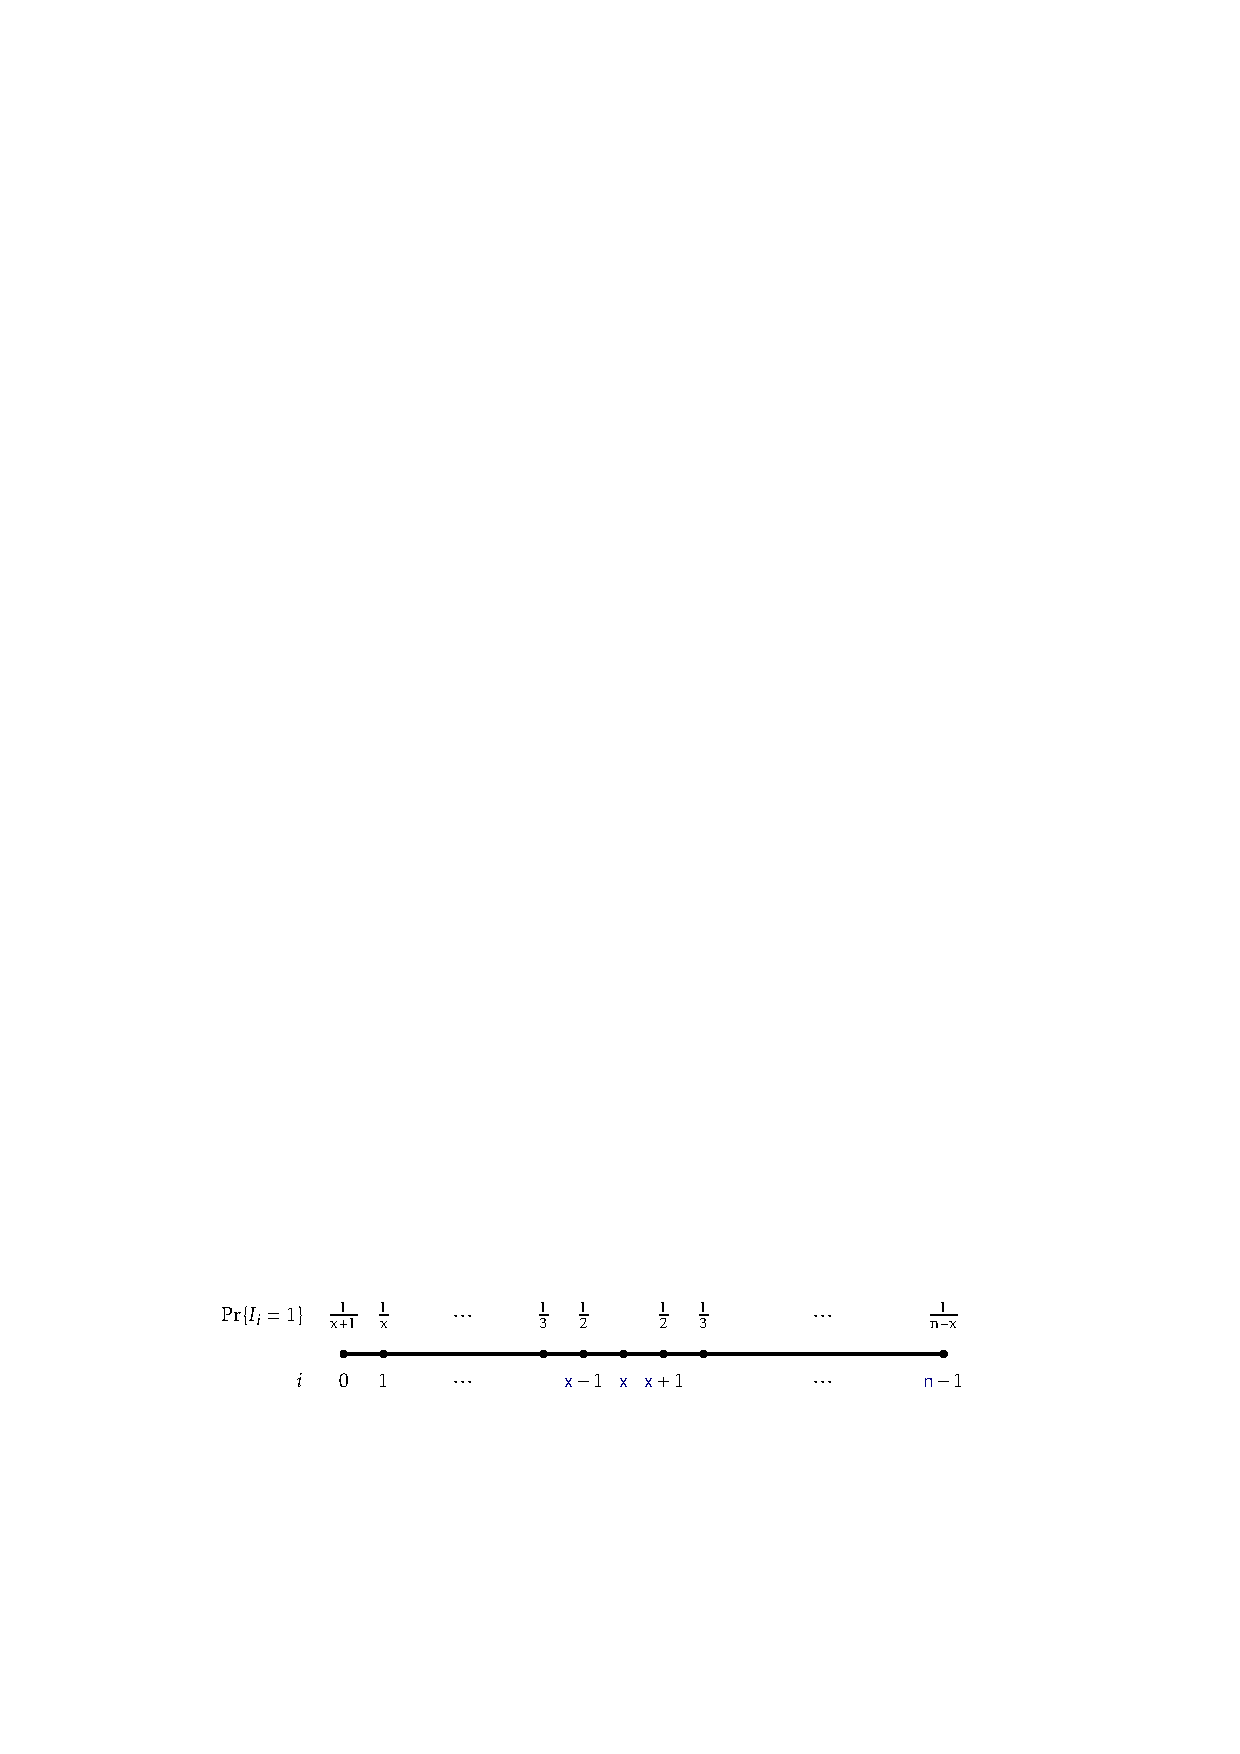
\includegraphics[width=\ScaleIfNeeded]{figs/rbst-probs-a} \\ (a) \\[2ex]
      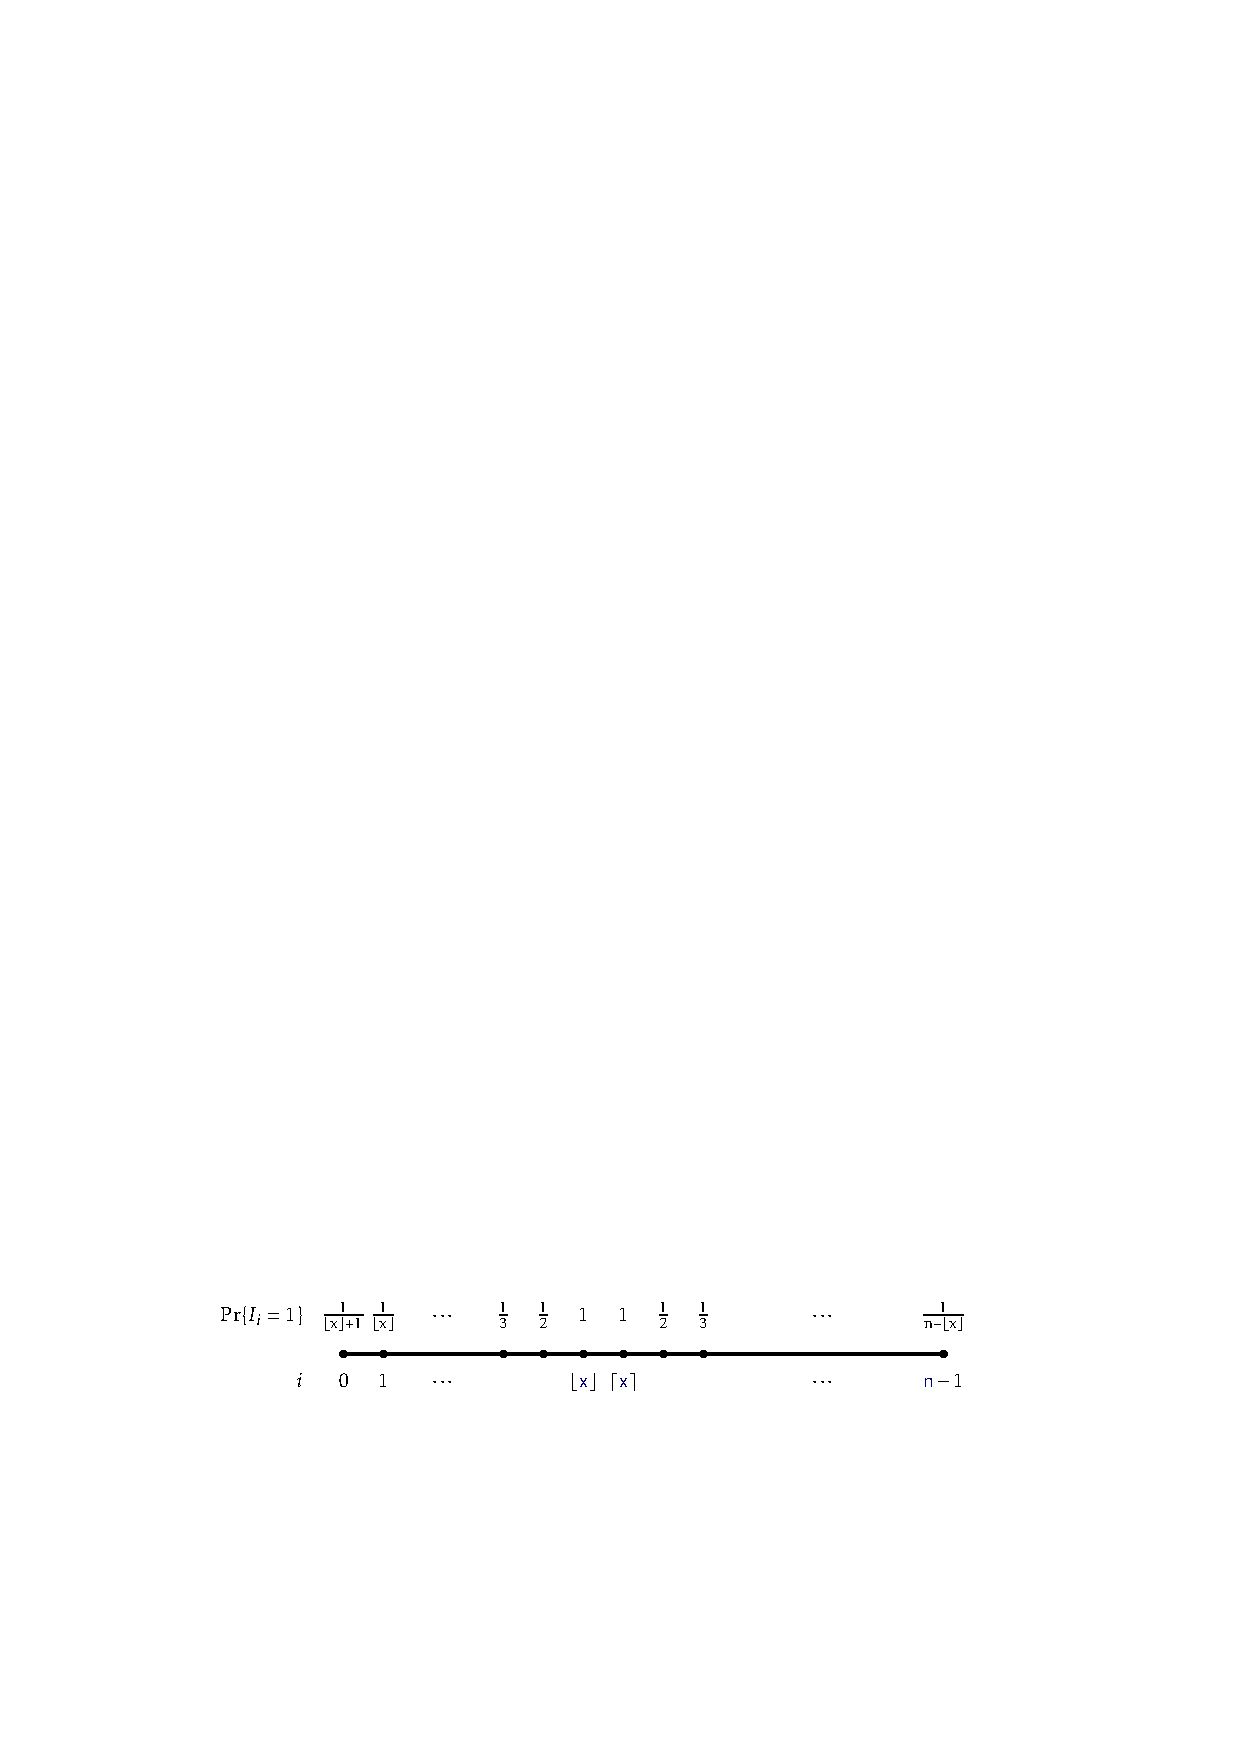
\includegraphics[width=\ScaleIfNeeded]{figs/rbst-probs-b} \\ (b) \\[2ex]
    \end{tabular}
  \end{center}
  \caption[As probabilidades de um elemento estar em um caminho de busca]{As probabilidades de um elemento estar no caminho de busca para #x#
   quando (a)~#x# é um inteiro e (b)~quando #x# não é um inteiro.}
  \figlabel{rbst-probs}
\end{figure}

\subsection{Resumo}

O teorema seguinte resume o desempenho de uma árvore binária aleatória de busca:

\begin{thm}\thmlabel{rbs}
Uma árvore binária aleatória de busca pode ser construída em um tempo $O(#n#\log #n#)$.
Em uma árvore binária aleatória de busca, a operação #find(x)# tem um tempo esperado de $O(\log #n#)$.
\end{thm}

Devemos enfatizar novamente que a expectativa no \thmref{rbs} é relativa
a uma permutação aleatória usada para criar a árvore binária aleatória de busca. Em particular, ela não depende de uma escolha aleatória de
#x#; ela é verdadeira para cada valor de #x#.


\section{#Treap#: Uma árvore Binária de Busca Aleatorizada}
\seclabel{treap}

\index{Treap@#Treap#}%
O problema com as árvores binárias aleatórias de buscas é, é claro, que elas não são
dinâmicas.  Elas não suportam as operações #add(x)# ou #remove(x)#
necessárias para implementar a interface #ConjuntoOrdenado#.  Nesta seção, descrevemos
uma estrutura de dados chamada #Treap# que usa o \lemref{rbs} para implementar
a interface #SSet#.\footnote{O nome #Treap# vem do fato 
que esta estrutura é, simultaneamente, uma árvore binária de busca (\textbf{tr}ee, em inglês) (\secref{binarysearchtree}) e um h\textbf{eap} (\chapref{heaps}).}

Um nó em uma #Treap# é como um nó em uma #ArvoreBinariaDeBusca# no sentido que
ele tem um valor para o dado, #x#, porém ele também tem uma \emph{prioridade},
numérica única, #p#, que é associada aleatoriamente:
\javaimport{ods/Treap.Node<T>}
\cppimport{ods/Treap.TreapNode}
Adicionalmente, para ser um árvore binária de busca, os nós de uma #Treap#
também obedecem à \emph{propriedade de heap}:
\begin{itemize}
\item (Propriedade de Heap)  Para cada nó #u#, exceto a raiz, 
      $#u.pai.p# < #u.p#$.
      \index{propriedade de heap}%
\end{itemize}
em outras palavras, cada nó possui uma prioridade menor que aquelas de seus dois filhos.
Um exemplo é mostrado na \figref{treap}.

\begin{figure}
  \begin{center}
    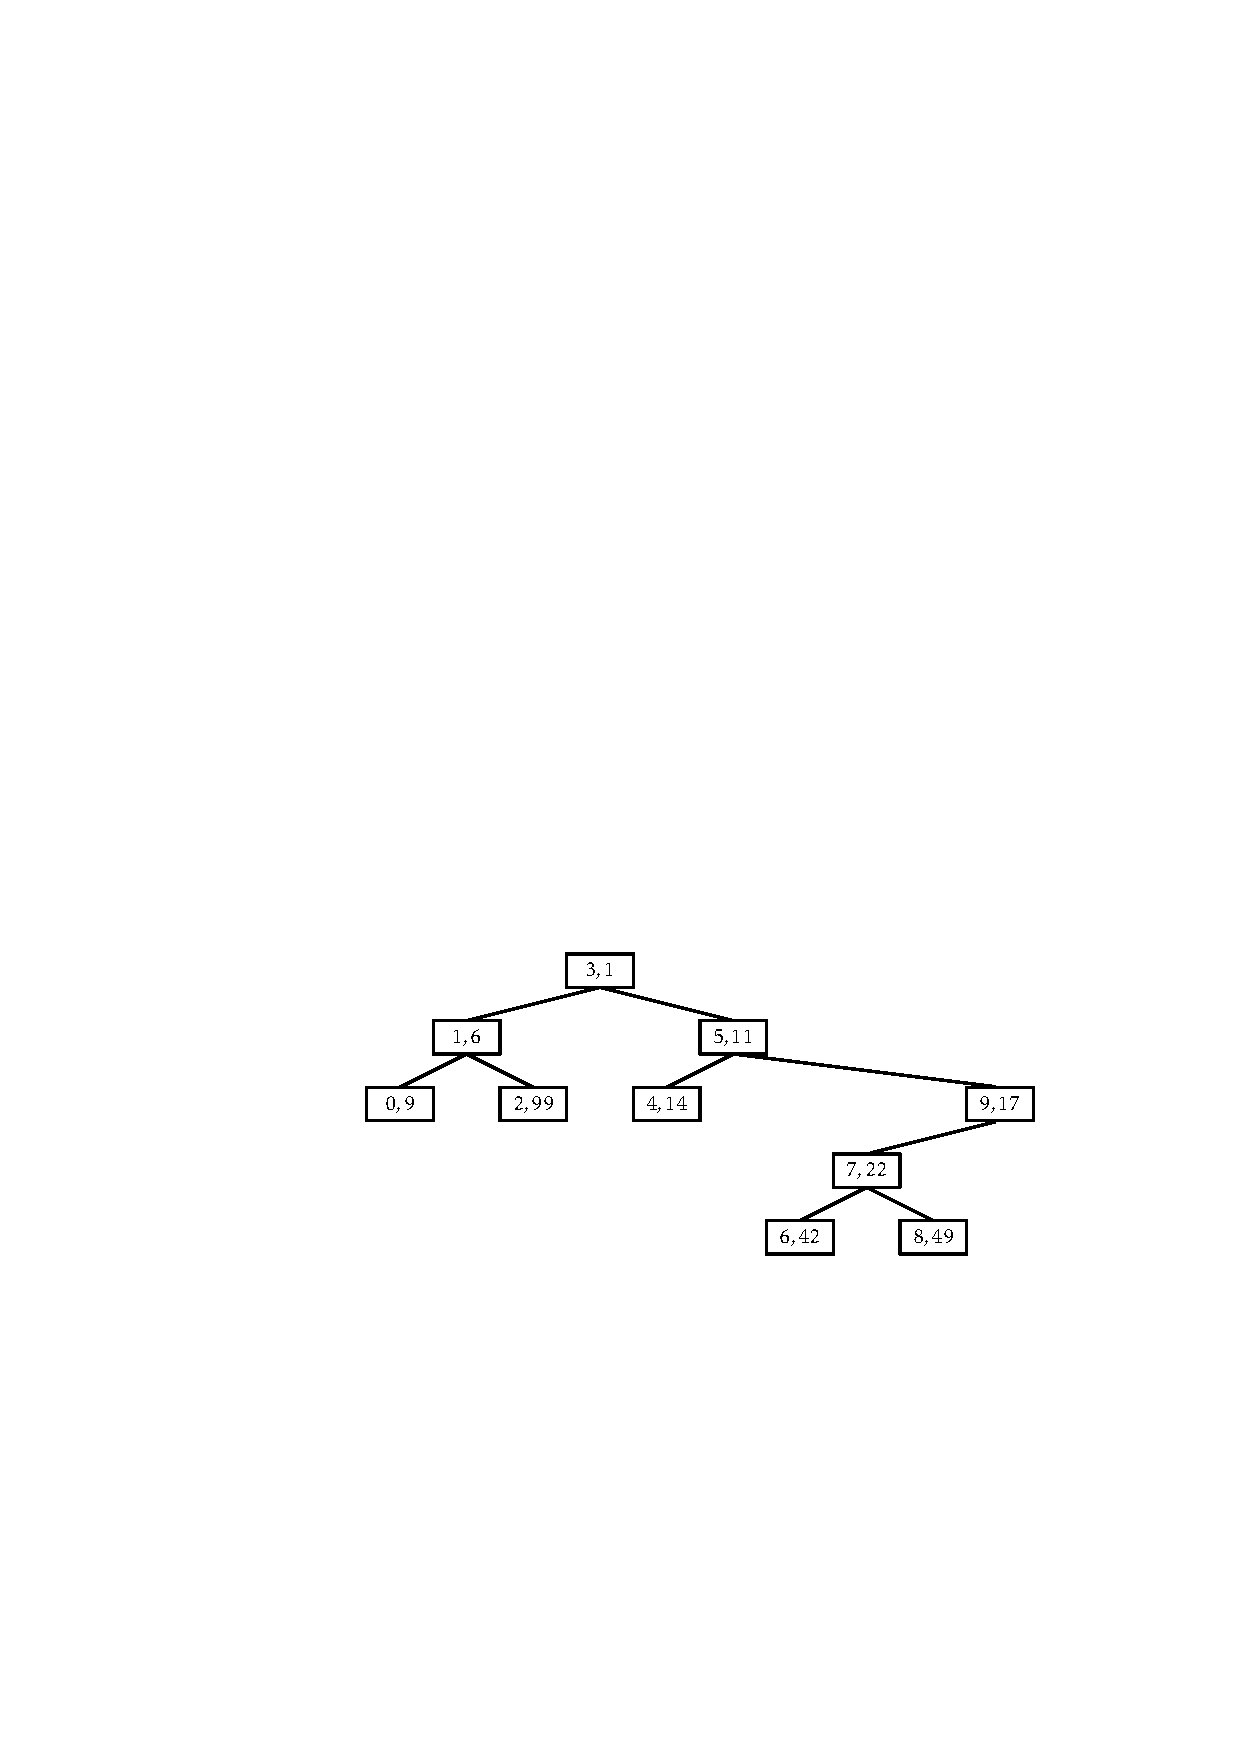
\includegraphics[width=\ScaleIfNeeded]{figs/treap}
  \end{center}
  \caption[Uma Treap]{Um exemplo de uma #Treap# contendo os inteiros
  $0,\ldots,9$. Cada nó, #u#, é ilustrado como uma caixa contendo $#u.x#,#u.p#$.}
  \figlabel{treap}
\end{figure}

As condições de heap e de árvore binária de busca juntas garantem que, uma vez
que a chave (#x#) e a prioridade (#p#) de cada nó seja definido, o formato
da #Treap# está completamente determinado. A propriedade de heap nos diz
que o nó com prioridade mínima tem que ser a raiz, #r#, da #Treap#.
A propriedade da árvore binária de busca nos diz que todos os nós com chaves menores
que #r.x# são armazenados na subárvore com raiz em #r.esquerdo# e todos os nós com
chaves maiores que #r.x# são armazenados na subárvore com raiz em #r.direito#.

Um ponto importante sobre os valores de prioridade em uma #Treap# é que eles
são únicos e atribuídos aleatoriamente.  Por conta disso, existem dois modos
equivalentes de pensar sobre uma #Treap#.  Como definido acima, uma
#Treap# obedece às propriedades do heap e da árvore binária de busca.  Alternativamente,
podemos pensar uma #Treap# como uma #ArvoreBinariaDeBusca# cujos nós
sejam inseridos em uma ordem crescente de prioridade.  Por exemplo, A #Treap#
na \figref{treap} pode ser obtida com a inserção da sequência de valores $(#x#,#p#)$
\[
  \langle
   (3,1), (1,6), (0,9), (5,11), (4,14), (9,17), (7,22), (6,42), (8,49), (2,99)
  \rangle
\]
em uma #ArvoreBinariaDeBusca#.

Como as prioridades são escolhidas aleatoriamente, isto é equivalente a pegar
uma permutação aleatória das chaves---neste caso a permutação é
\[
  \langle 3, 1, 0, 5, 9, 4, 7, 6, 8, 2 \rangle
\]
---e inserindo essas em uma #ArvoreBinariaDeBusca#.  Porém isso significa que a
forma de uma treap é idêntica àquela de uma árvore binária aleatória de busca.
Particularmente, se substituirmos cada chave #x# por sua posição,\footnote{A
posição de um elemento #x# em um conjunto de elementos $S$ é o número de
elementos em $S$ que são menores que #x#.} então o \lemref{rbs} é válido.
Redeclarando o \lemref{rbs} em termos de uma #Treap#s, temos:
\begin{lem}\lemlabel{rbs-treap}
  Em uma #Treap# que armazena um conjunto $S$ de #n# chaves, as seguintes declarações são verdadeiras:
  \begin{enumerate}
    \item Para qualquer $#x#\in S$, o tamanho esperado do
    caminho de busca para #x# é $H_{r(#x#)+1} + H_{#n#-r(#x#)} - O(1)$.
    \item Para qualquer $#x#\not\in S$, o tamanho esperado do
        caminho de busca para #x# é $H_{r(#x#)} + H_{#n#-r(#x#)}$.
  \end{enumerate}
  Aqui, $r(#x#)$ indica a posição #x# no conjunto $S\cup\{#x#\}$.
\end{lem}
Novamente, enfatizamos que a expectativa no \lemref{rbs-treap} é tirada
sobre as escolhas aleatórias das prioridades de cada nó.  Ela não requer
qualquer pressuposto sobre a aleatoriedade nas chaves.

O \lemref{rbs-treap} nos diz que #Treap#s pode implementar a operação #find(x)#
eficientemente. Contudo, o benefício real de uma #Treap# é que ela pode 
suportar as operações #add(x)# e #delete(x)#.  Para
fazer isto, ela precisa executar rotações de modo a manter 
a propriedade de heap.  Veja a \figref{rotations}.
Uma \emph{rotação}
\index{rotação}%
em uma árvore binária de busca
é uma modificação local que pega um pai #u# de um nó #w#
e torna #w# o pai de #u#, enquanto preserva a propriedade da árvore binária de busca.
 Rotações vêm com dois sabores: \emph{à esquerda} or \emph{à direita}
dependendo se #w# é um filho direito ou esquerdo de #u#, respectivamente.
\index{rotação à esquerda}%
\index{rotação à direita}%

\begin{figure}
  \begin{center}
     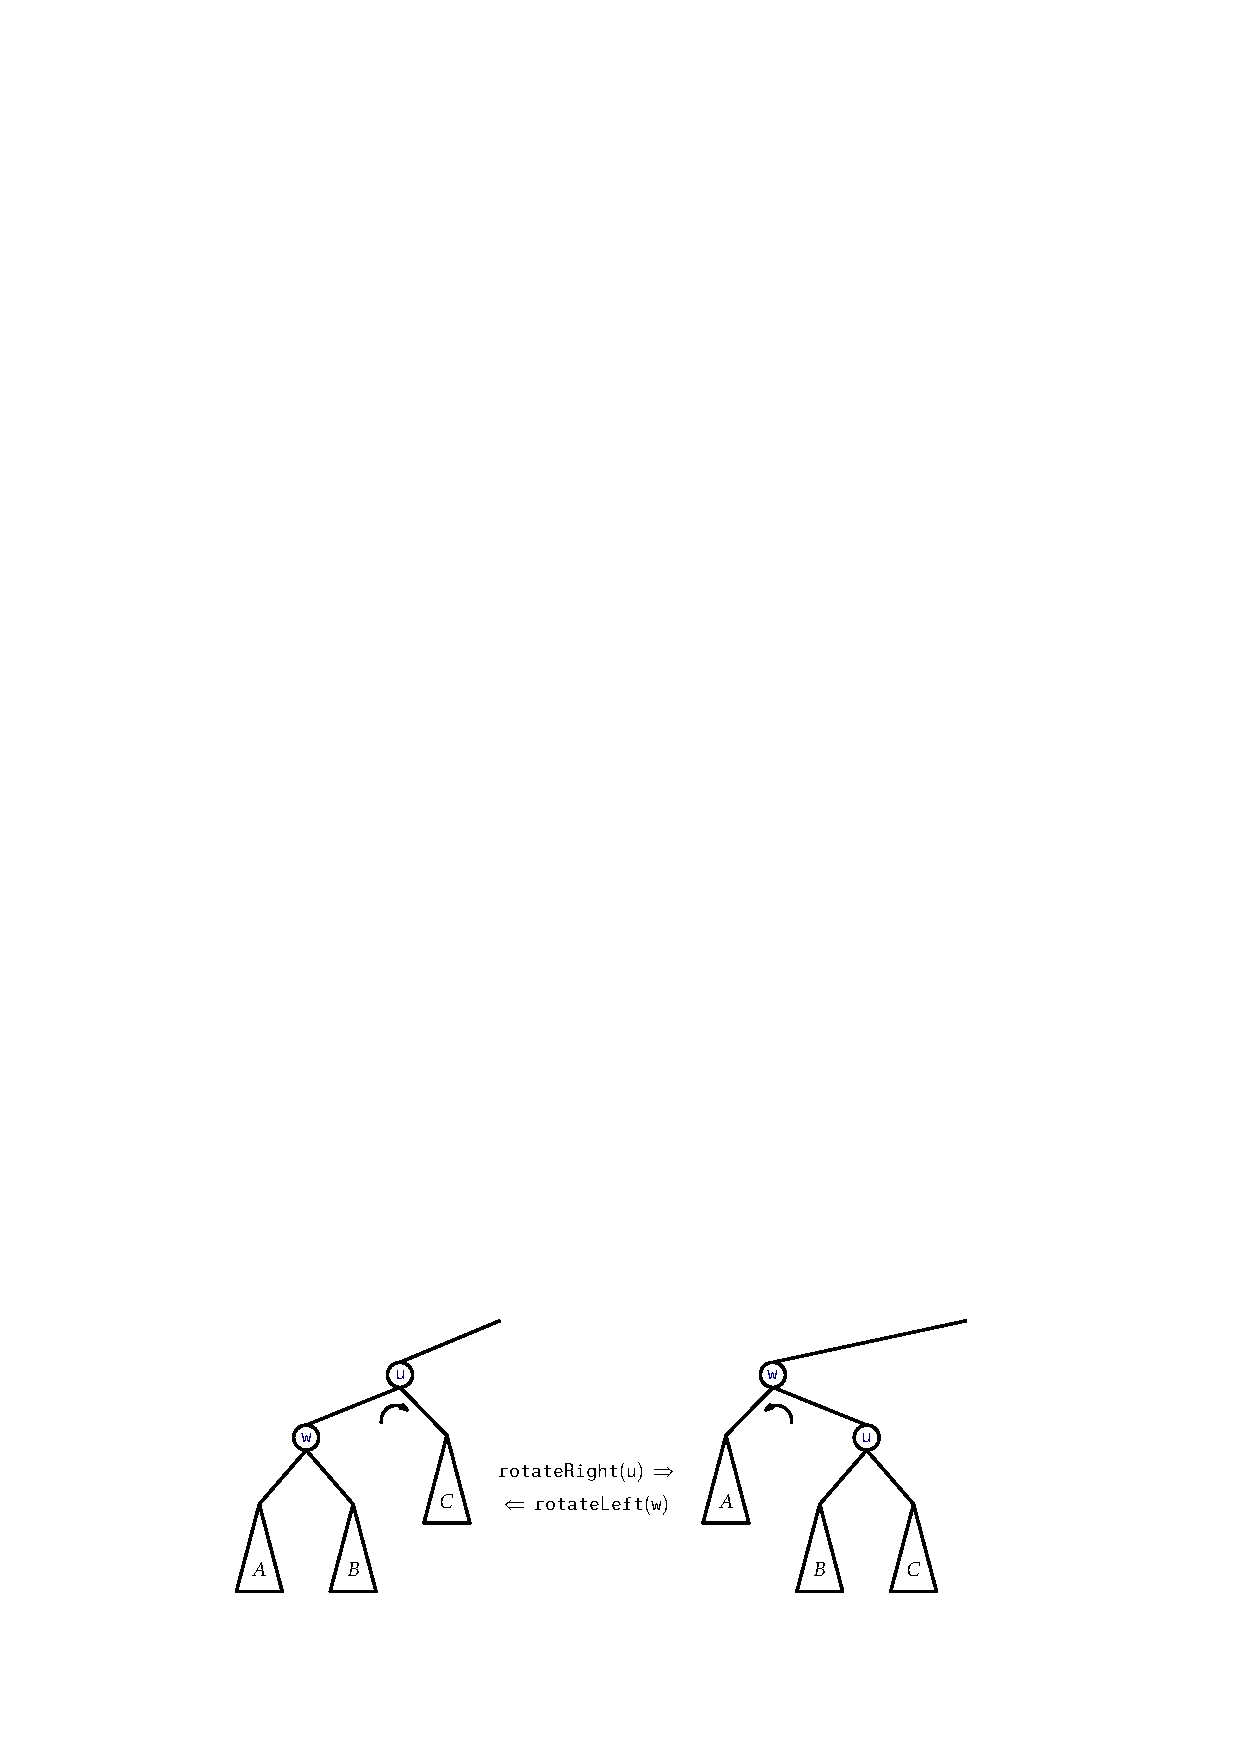
\includegraphics[width=\ScaleIfNeeded]{figs/rotation}
  \end{center}
  \caption{Rotações à esquerda e à direita em uma árvore binária de busca.}
  \figlabel{rotations}
\end{figure}

O código que implementa isto deve prever essas duas possibilidades e
tomar cuidado com um caso limite (quando #u# é a raiz), deste modo, o código real
é um pouco mais longo que a \figref{rotations} poderia levar um leitor a crer:
\codeimport{ods/BinarySearchTree.rotateLeft(u).rotateRight(u)}
\label{page:rotations}
Em termos da estrutura de dados #Treap#, a propriedade mais importante de uma
rotação é que a profundidade de #w# diminui de um enquanto a profundidade de #u#
aumenta de um.

Usando rotações, podemos implementar a operação #add(x)# como se segue:
Criamos um novo nó, #u#, atribuímos #u.x=x#, e escolhemos um valor aleatório
para #u.p#.  Em seguida, inserimos #u# usando o algoritmo usual #add(x)# 
para uma #ArvoreBinariaDeBusca#, assim, #u# agora é uma nova folha de #Treap#.
Neste ponto, nossa #Treap# satisfaz a propriedade da árvore binária de busca,
mas não necessariamente a propriedade de heap.  Particularmente, pode ser 
o caso em que #u.pai.p > u.p#.  Se este é o caso, então executamos uma
rotação no nó #w#=#u.pai# de modo que #u# se torne o pai de #w#.
Se #u# continua a violar a propriedade de heap, teremos que repetir isso, 
diminuindo a profundidade de #u# por um a cada vez, até
que #u# se torne a raiz ou $#u.pai.p# < #u.p#$.
\codeimport{ods/Treap.add(x).bubbleUp(u)}
Um exemplo de uma operação #add(x)# é mostrada na \figref{treap-add}.

\begin{figure}
  \begin{center}
  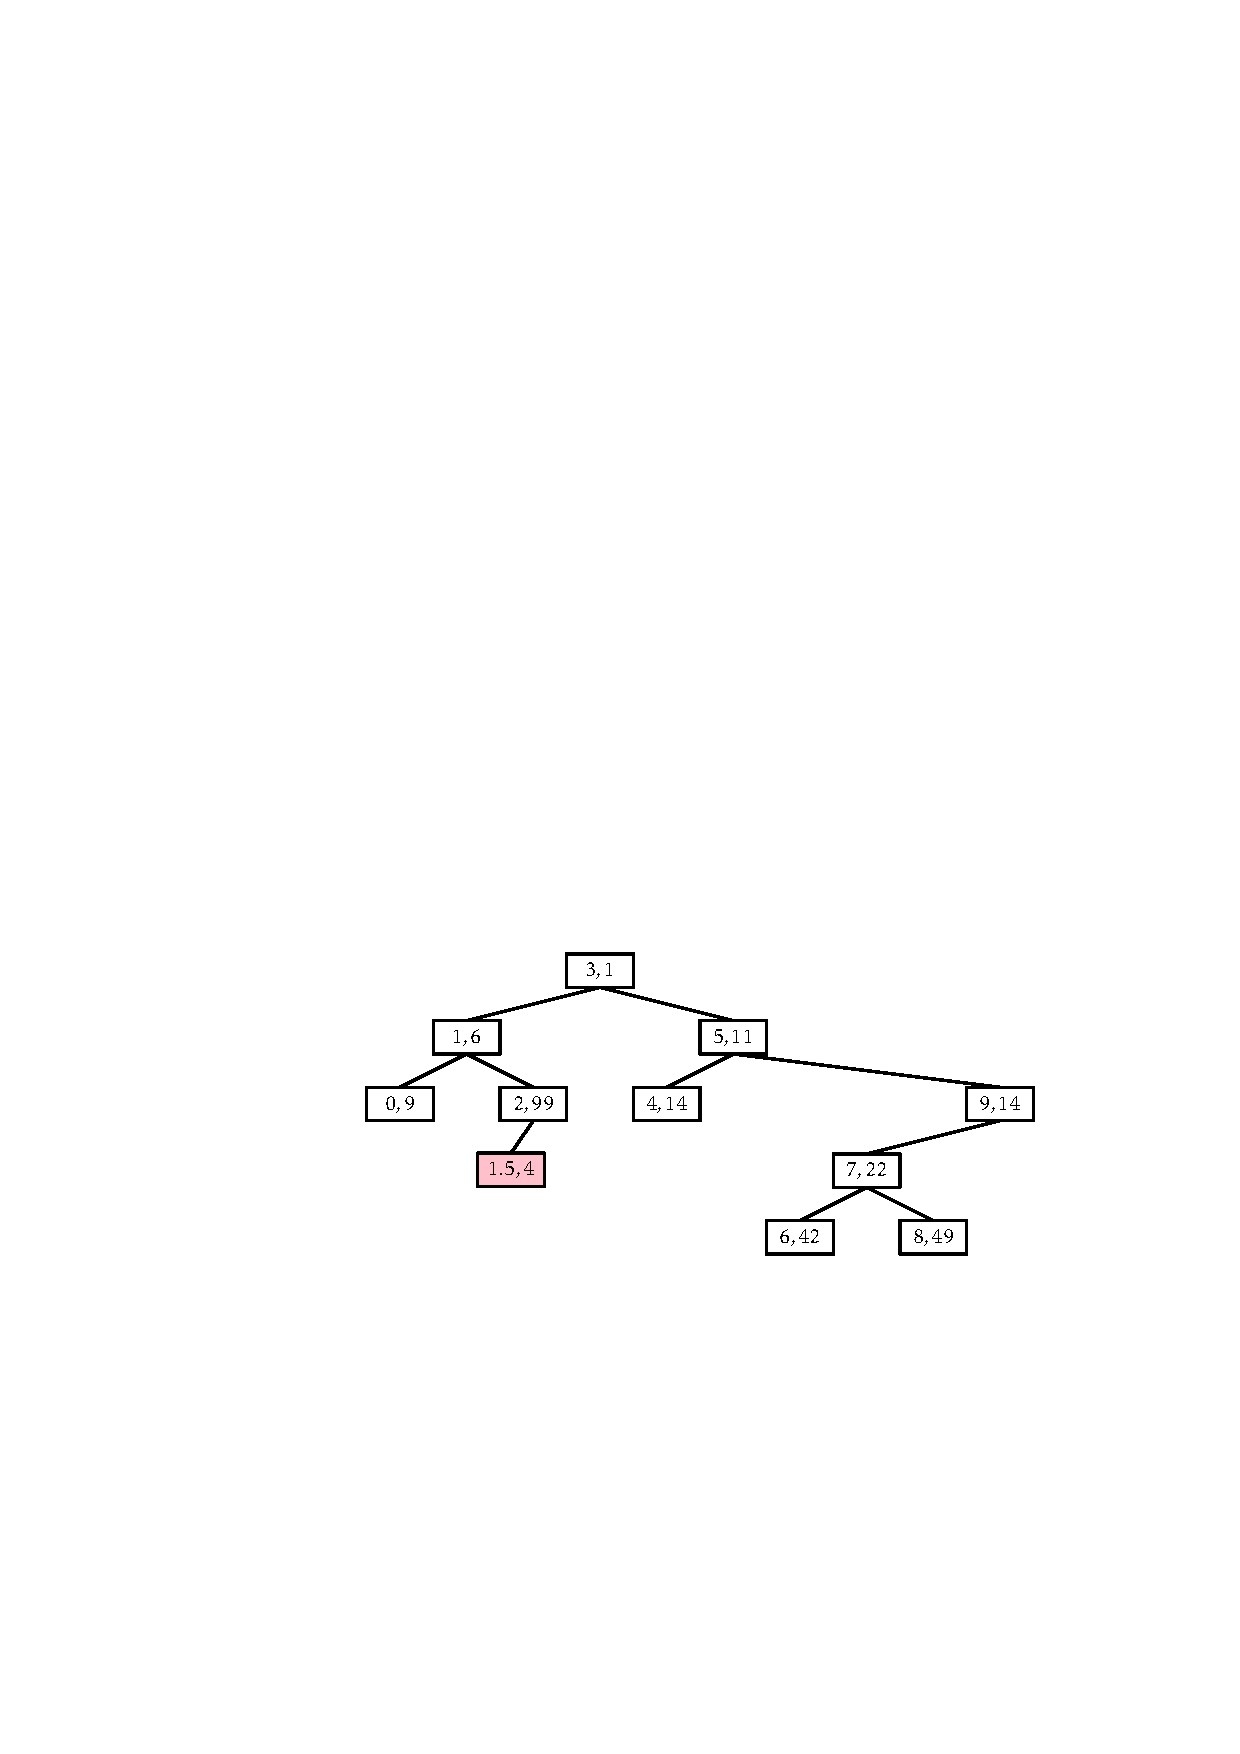
\includegraphics[width=\ScaleIfNeeded]{figs/treap-insert-a} \\
  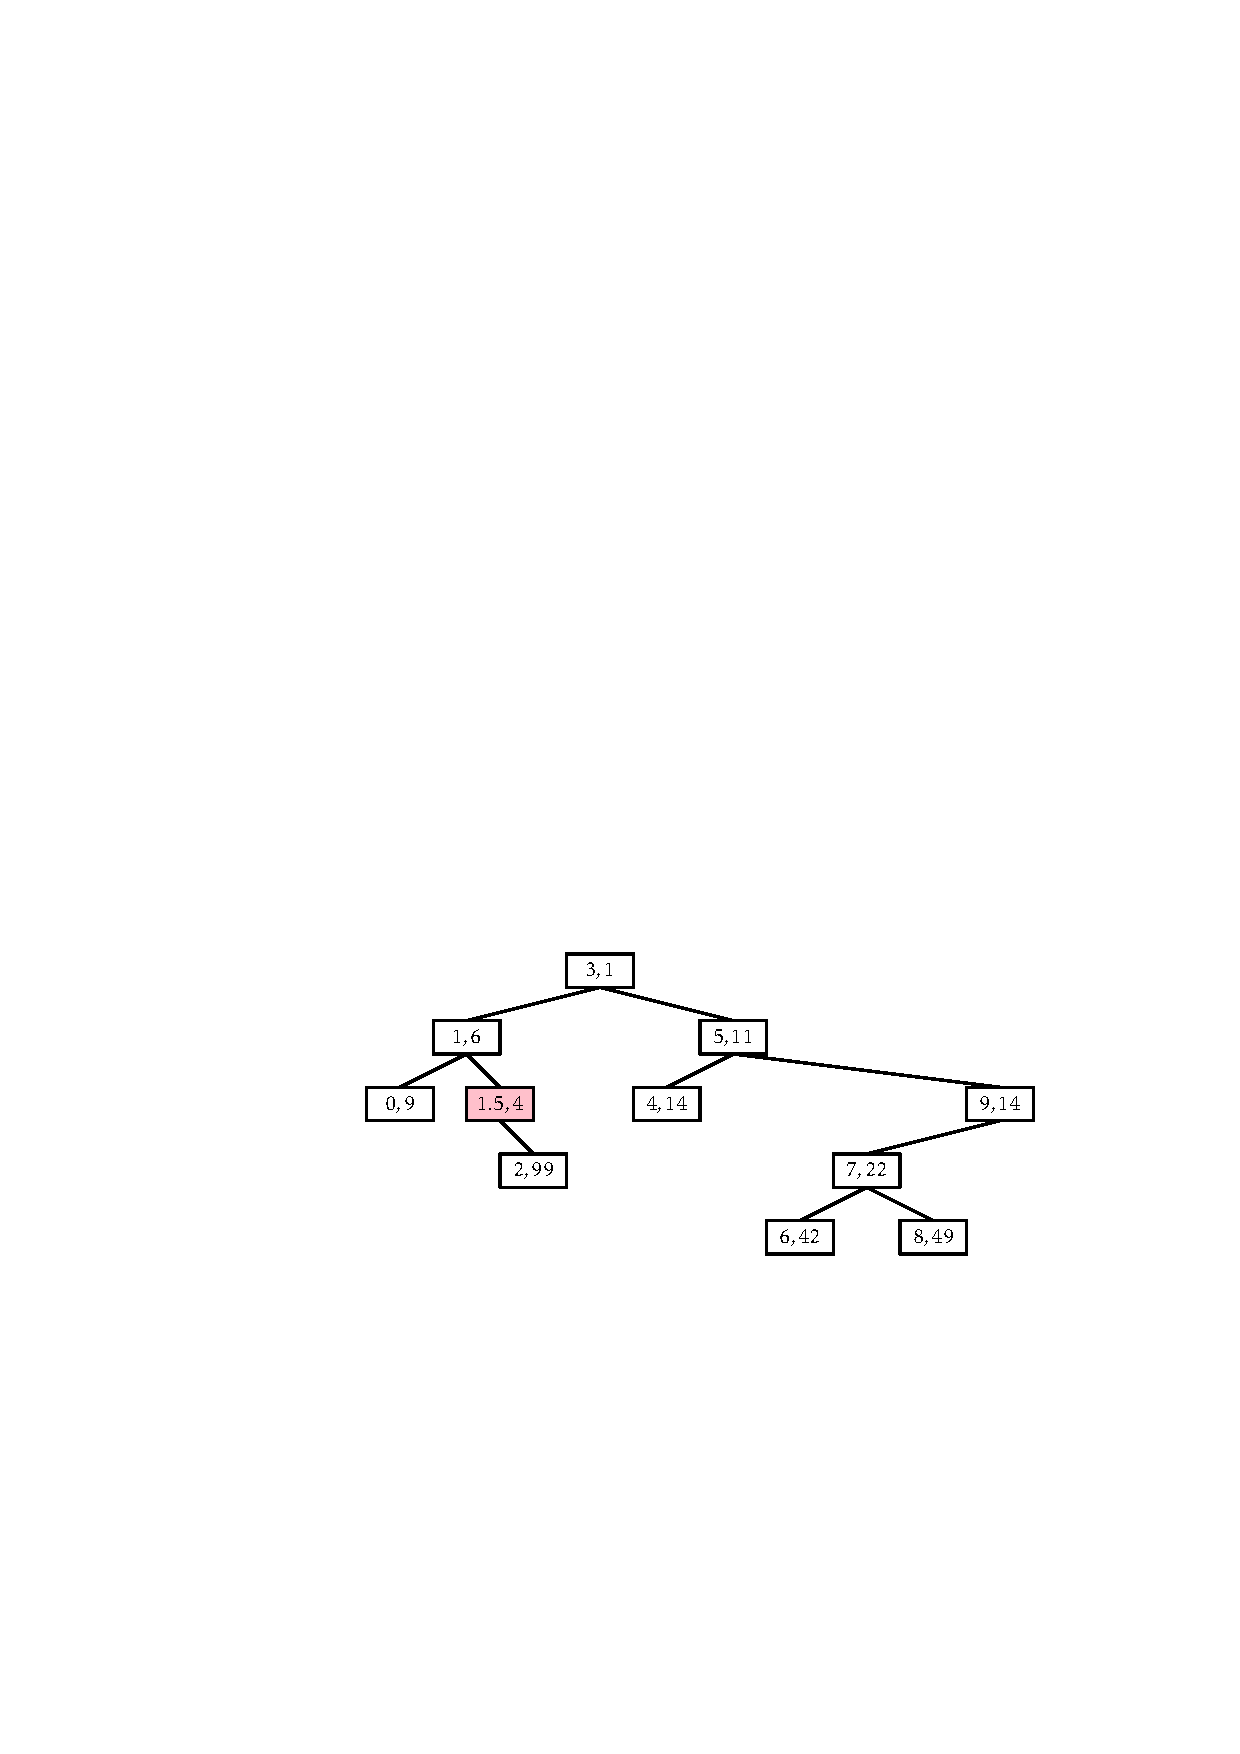
\includegraphics[width=\ScaleIfNeeded]{figs/treap-insert-b} \\
  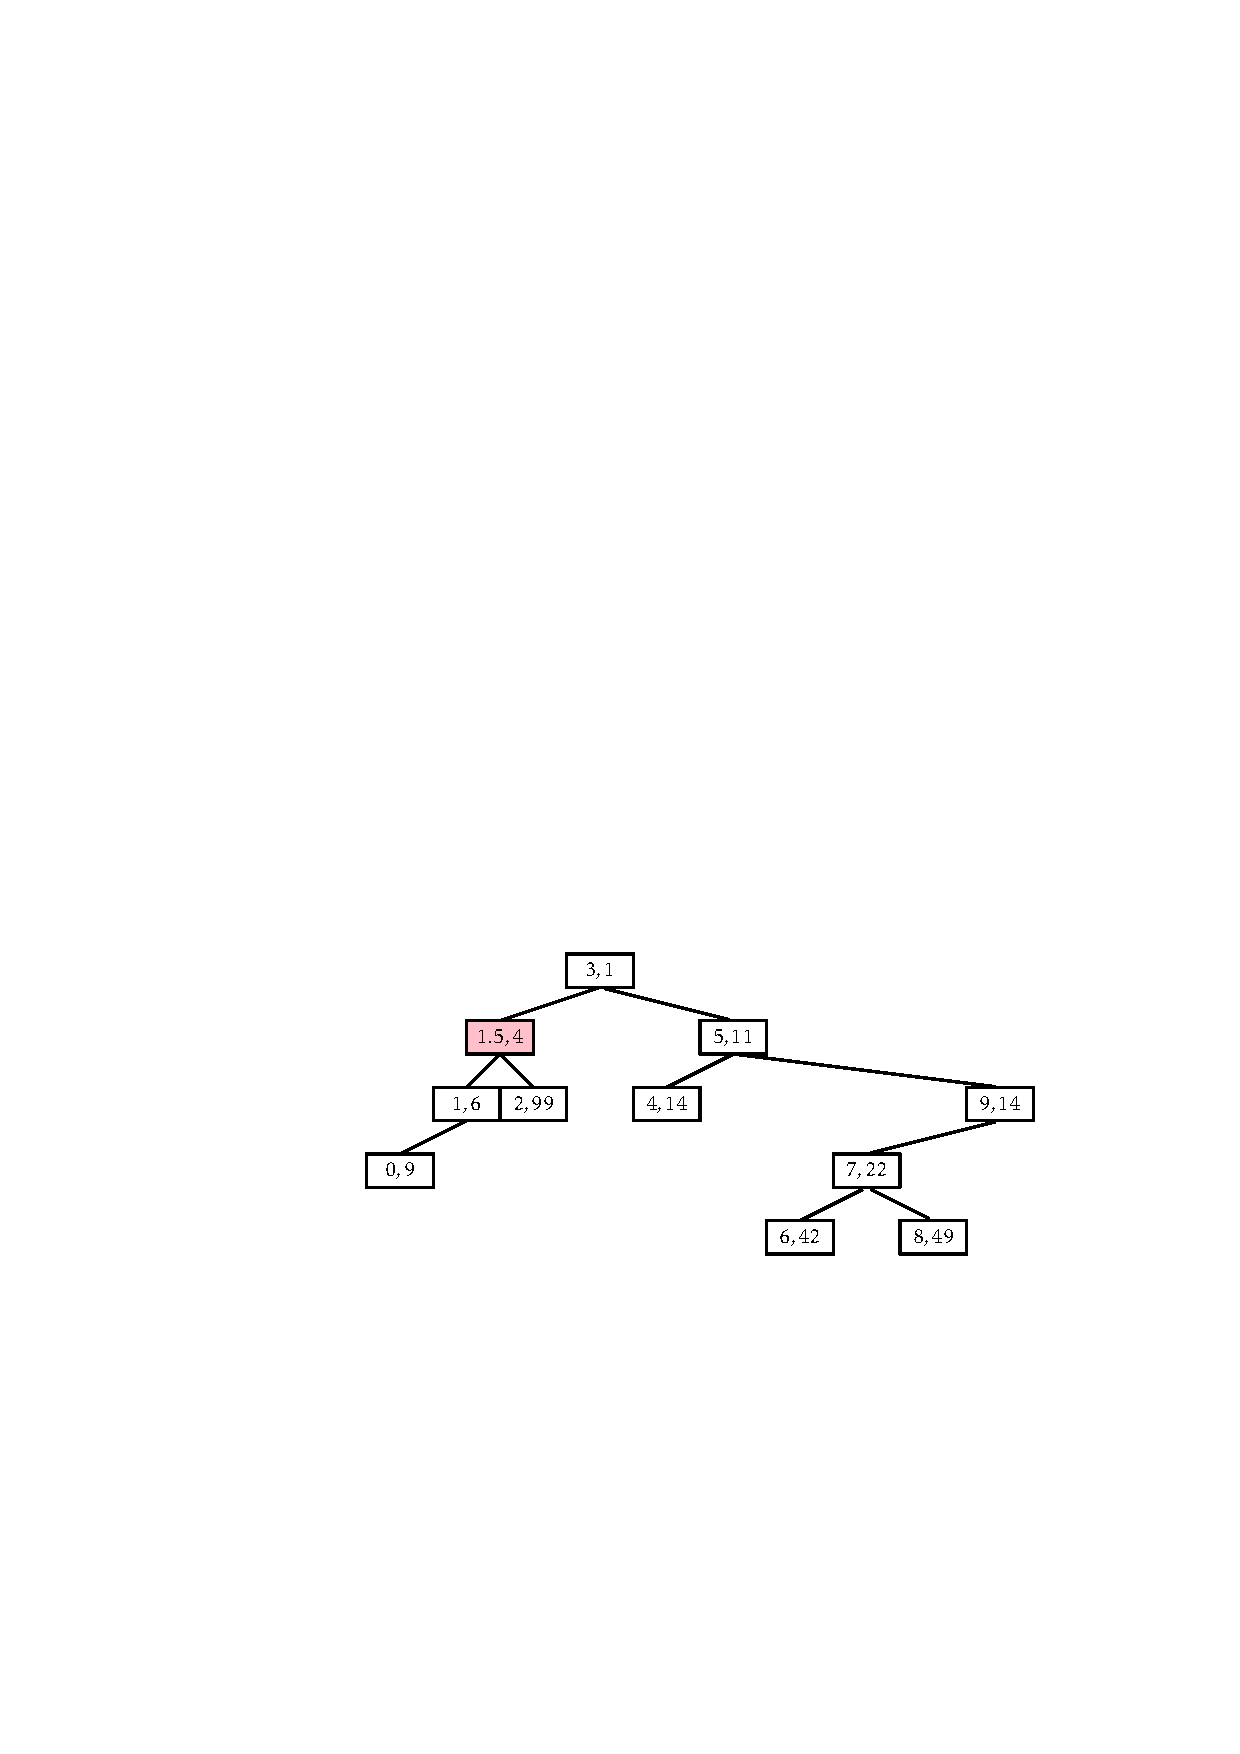
\includegraphics[width=\ScaleIfNeeded]{figs/treap-insert-c} \\
  \end{center}
  \caption[Inserindo em uma Treap]{Inserindo o valor 1.5 na #Treap# da \figref{treap}.}
  \figlabel{treap-add}
\end{figure}

O tempo de execução de uma operação #add(x)# é dado pelo tempo 
que leva para seguir o caminho de busca para #x# mais o número de rotações
executadas para mover o nó recém adicionado, #u#, na sua localização correta
na #Treap#.  Pelo \lemref{rbs-treap}, o comprimento esperado do
caminho de busca é no máximo $2\ln #n#+O(1)$.  Além disso, cada rotação
diminui a profundidade de #u#.   Esse processo cessa se #u# se torna a raiz, assim
o número esperado de rotações não pode ultrapassar o comprimento esperado
do caminho de busca.  Então, o tempo esperado de execução da operação #add(x)#
em uma #Treap# é $O(\log #n#)$.  (O \excref{treap-rotates}
pede para demonstrar que o número esperado de rotações executadas durante
uma inserção é, de fato, somente $O(1)$.)

A operação #remove(x)# em uma #Treap# é o oposto da operação #add(x)#.
Procuramos pelo nó, #u#, contendo #x#, então executamos
rotações para mover #u# para baixo até que ele se torne uma folha, e então separamos
#u# da #Treap#.  Note que, para mover #u# para baixo, podemos
executar ou uma rotação para esquerda ou uma pra direita em #u#, que vai substituir #u#
por #u.direito# ou #u.esquerdo#, respectivamente.
A escolha é feita de acordo com a primeira situação seguinte que aparece:
\begin{enumerate}
\item Se #u.esquerdo# e #u.direito# são ambos #null#, então #u# é uma folha e nenhuma rotação é feita.
\item Se #u.esquerdo# (ou #u.direito#) é #null#, então executamos uma rotação à direita (ou à esquerda, respectivamente) em #u#.
\item Se $#u.esquerdo.p# < #u.direito.p#$ (ou $#u.esquerdo.p# > #u.direito.p#)$, então executamos uma rotação à direita (ou rotação à esquerda, respectivamente) em #u#.
\end{enumerate}
Essas três regras asseguram que a #Treap# não se torne desconectada e que a 
propriedade de heap seja restabelecida uma vez que #u# seja removido.
\codeimport{ods/Treap.remove(x).trickleDown(u)}
Um exemplo da operação #remove(x)# é mostrado na \figref{treap-remove}.
\begin{figure}
  \begin{center}
  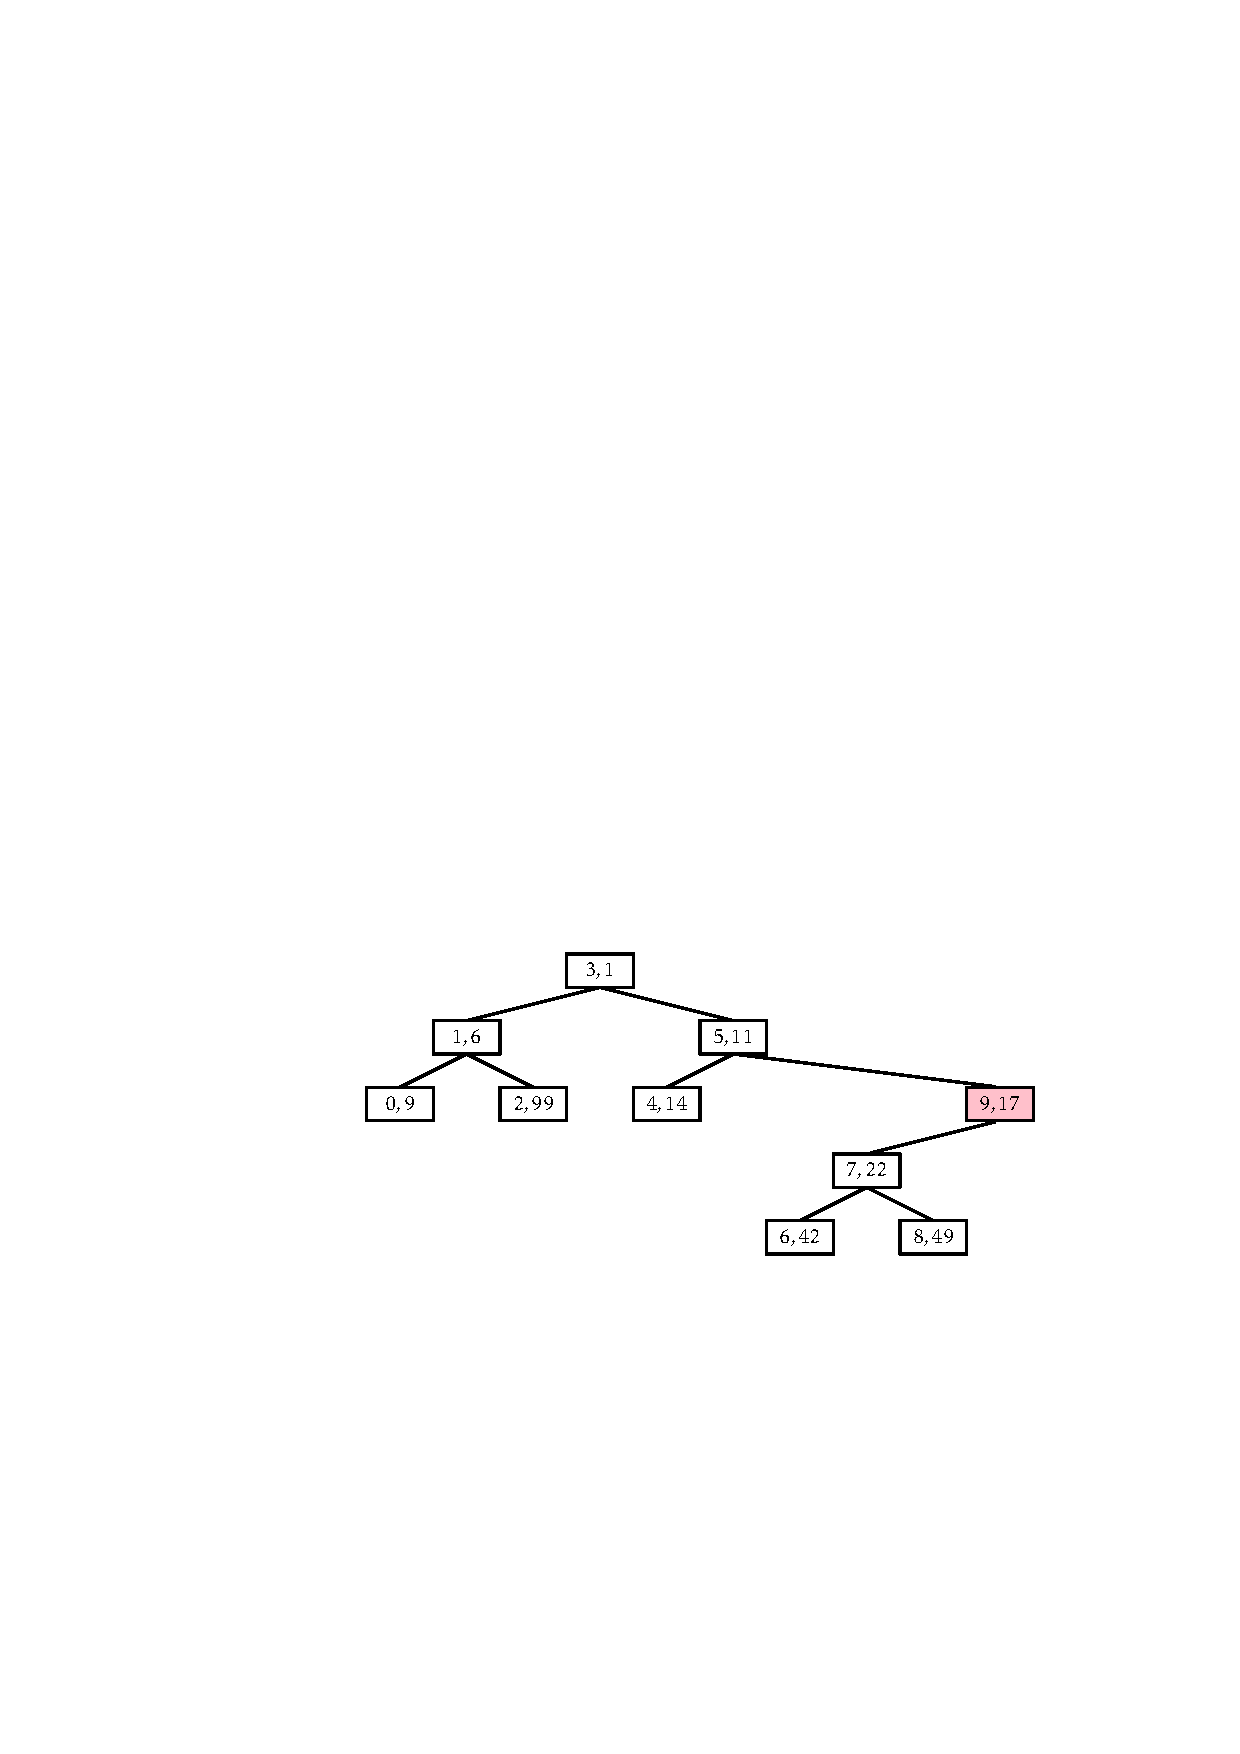
\includegraphics[height=\QuarterHeightScaleIfNeeded]{figs/treap-delete-a} \\
  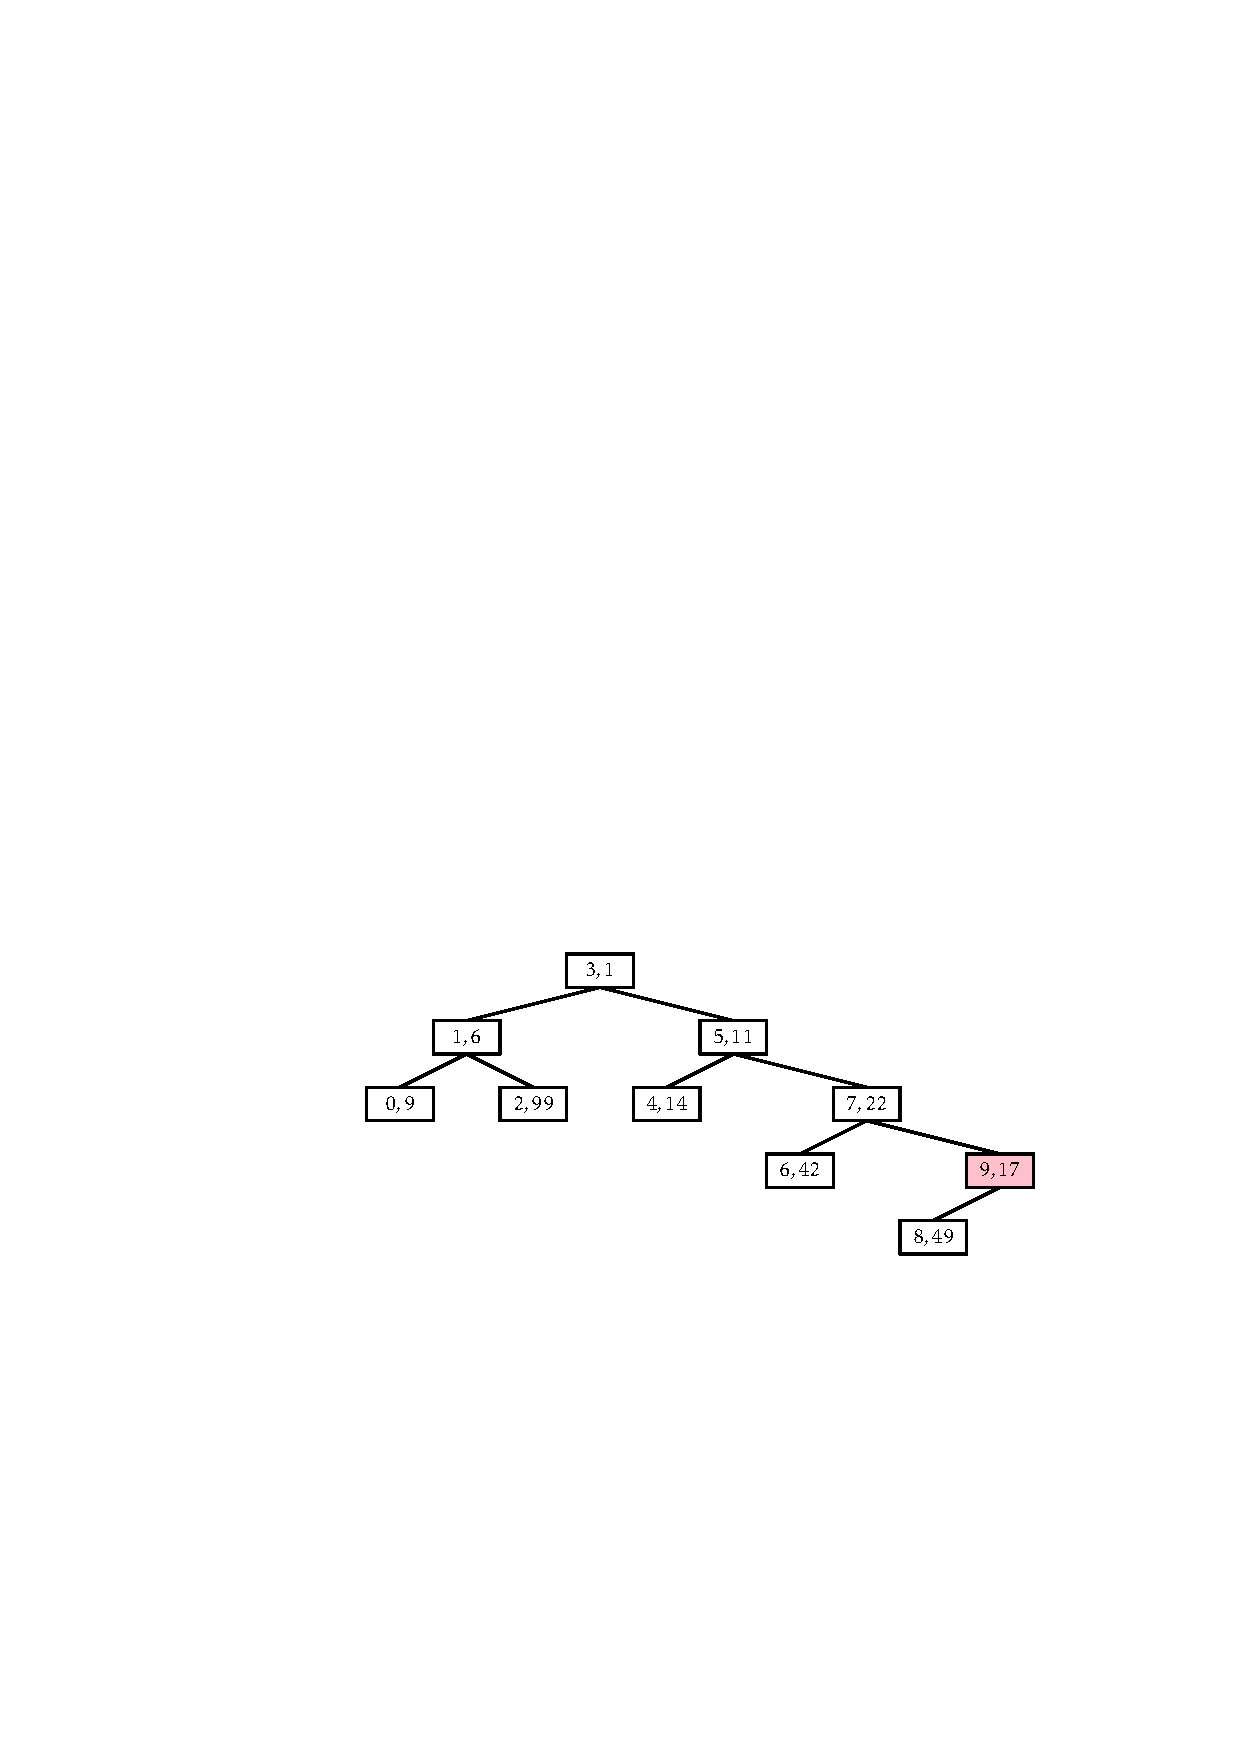
\includegraphics[height=\QuarterHeightScaleIfNeeded]{figs/treap-delete-b} \\
  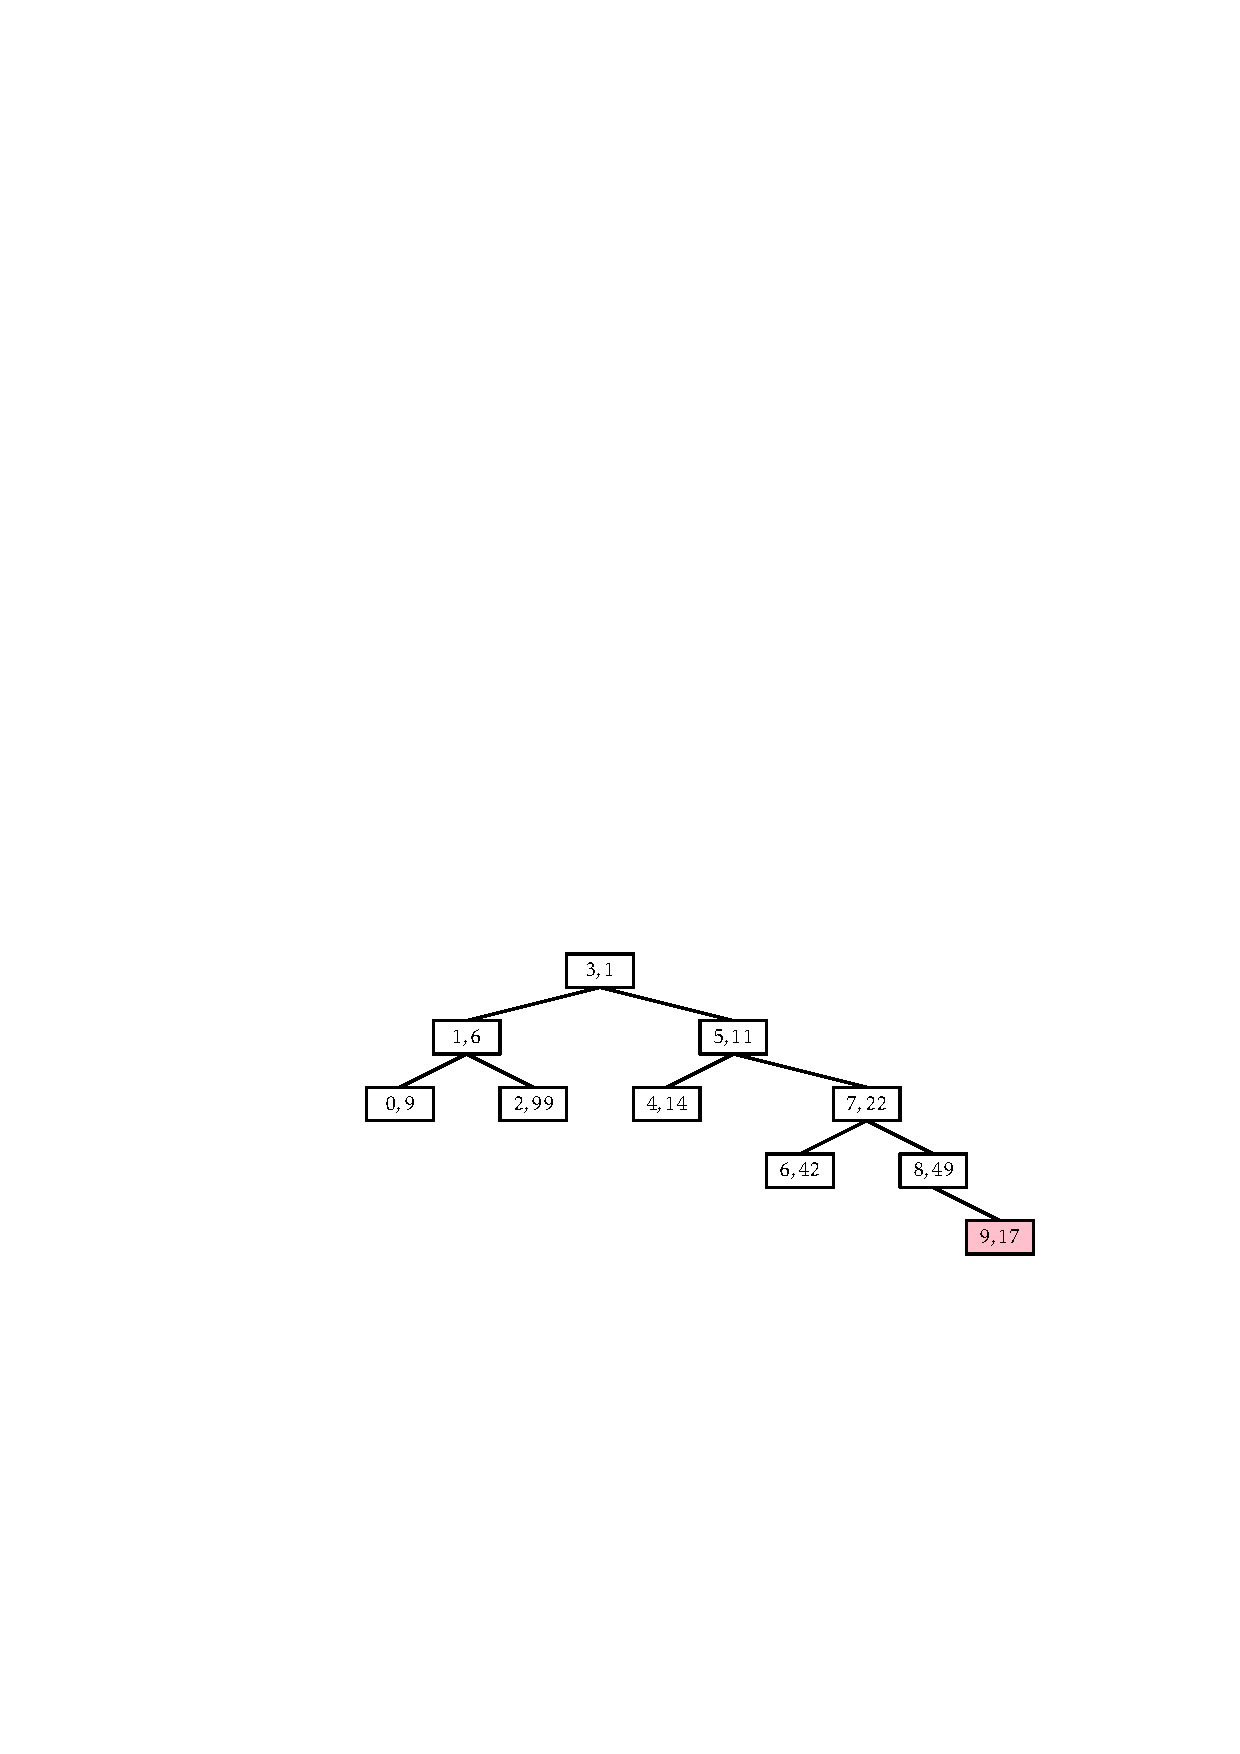
\includegraphics[height=\QuarterHeightScaleIfNeeded]{figs/treap-delete-c} \\
  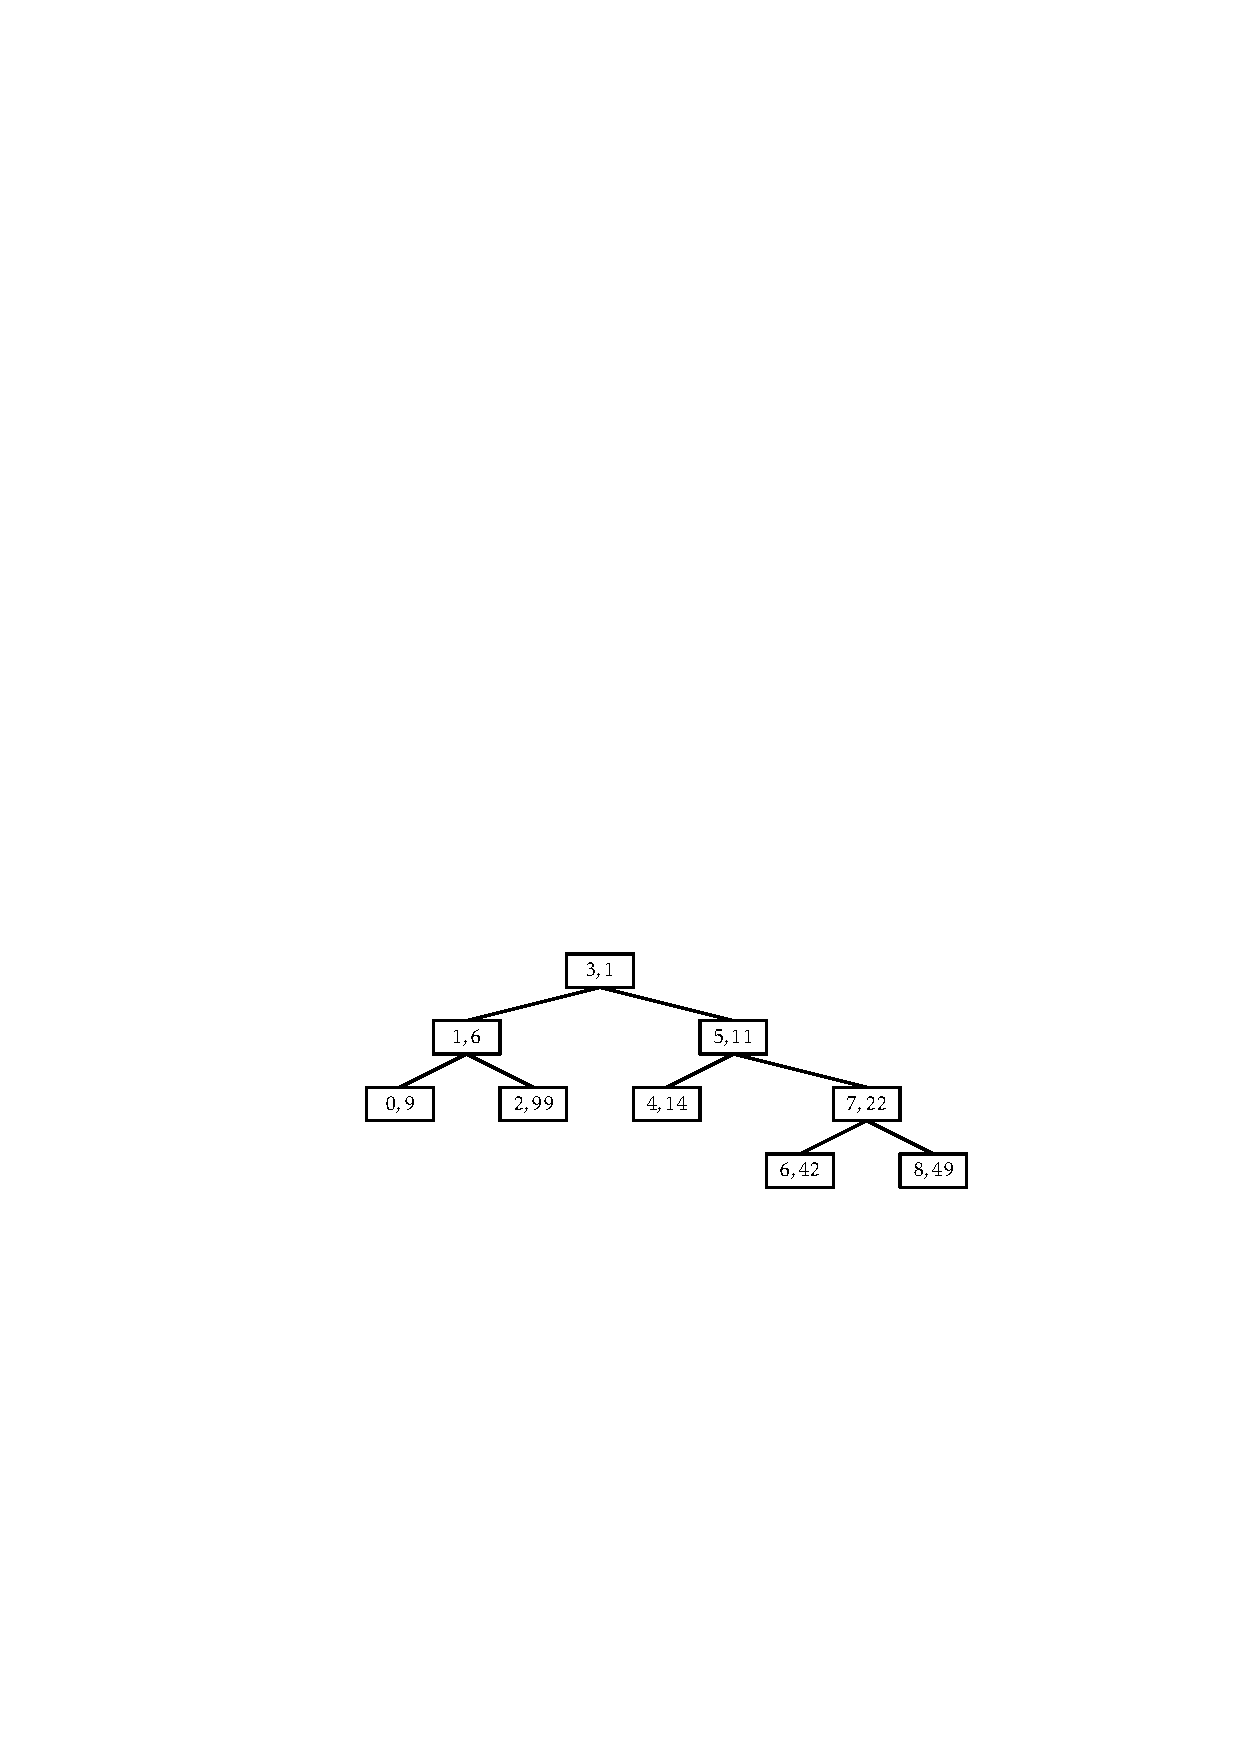
\includegraphics[height=\QuarterHeightScaleIfNeeded]{figs/treap-delete-d} 
  \end{center}
  \caption[Removendo de uma treap]{Removendo o valor 9 da #Treap# na \figref{treap}.}
  \figlabel{treap-remove}
\end{figure}

O truque para analisar o tempo de execução da operação #remove(x)# é
notar que a operação inverte a operação #add(x)#.
Particularmente, se reinserimos #x#, usando a mesma prioridade #u.p#,
então a operação #add(x)# faria exatamente o mesmo número de rotações
e iria restabelecer a #Treap# para exatamente o mesmo estado em que estava antes 
da operação #remove(x)# ter sido executada.  (Lendo de baixo para cima, a
\figref{treap-remove} ilustra a inserção do valor 9 em uma
#Treap#.) Isto significa que o tempo de execução esperado de #remove(x)#
em uma #Treap# de tamanho #n# é proporcional ao tempo esperado de execução
da operação #add(x)# em uma #Treap# de tamanho $#n#-1$.  Concluímos
que o tempo esperado de execução de #remove(x)# é $O(\log #n#)$.

\subsection{Resumo}

O teorema seguinte resume o desempenho de uma estrutura de dados #Treap#:

\begin{thm}
Uma #Treap# implementa a interface #SSet#. Uma #Treap# suporta
as operações #add(x)#, #remove(x)#, e #find(x)# em um tempo esperado de $O(\log #n#)$
por operação.
\end{thm}

Vale a pena comparar a estrutura de dados #Treap# a uma estrutura de dados 
#SkiplistSSet#.  Ambas implementam as operações #SSet# em um tempo esperado 
de $O(\log #n#)$ por operação.  Em ambas estruturas de dados, #add(x)# e
#remove(x)# envolvem uma busca e então um número constante de mudanças em ponteiros
(veja \excref{treap-rotates} abaixo).  Assim, para ambas as estruturas,
o comprimento esperado do caminho de busca é o valor crítico para valiar
seus desempenhos.  Em uma #SkiplistSSet#, o comprimento esperado de um
caminho de busca é
\[
     2\log #n# + O(1) \enspace ,
\]
Em uma #Treap#, o comprimento esperado de um caminho de busca é
\[
    2\ln #n# +O(1) \approx 1.386\log #n#  + O(1) \enspace .
\]
Assim, os caminhos de busca em uma #Treap# são consideravelmente menores e isto se
traduz em operações notadamente mais rápidas em uma #Treap#s que em uma #Skiplist#s.
O \excref{skiplist-opt} no \chapref{skiplists} mostra como
o comprimento esperado de um caminho de busca em uma #Skiplist# pode ser
reduzido para
\[
     e\ln #n# + O(1) \approx 1.884\log #n# + O(1) 
\]
usando o lançamento de uma moeda viciada.  Mesmo com esta otimização, o comprimento
esperado dos caminhos de busca em uma #SkiplistSSet# é notadamente mais longo que
em uma #Treap#.

\section{Discussão e Exercícios}

Árvores binárias de buscas aleatórias foram estudadas extensivamente.  Devroye
\cite{d88} fornece uma prova do \lemref{rbs} e resultados relacionados. Existem 
resultados muito mais fortes na literatura, o mais impressionante
dos quais é devido a Reed \cite{r03}, que mostra que a altura esperada de uma
árvore binária aleatória de busca é
\[
  \alpha\ln n - \beta\ln\ln n + O(1)
\]
onde $\alpha\approx4.31107$ é o valor da solução única no intervalo
$[2,\infty)$ da equação $\alpha\ln((2e/\alpha))=1$ e
$\beta=\frac{3}{2\ln(\alpha/2)}$ .  Além disso, a variância da altura é constante.

O nome #Treap# foi criado por Seidel e Aragon \cite{as96} que discutiram
#Treap#s e algumas de suas variantes.  Contudo, a estrutura básica foi
estudada anteriormente por Vuillemin \cite{v80} que as chamou de árvores Cartesinas.

Uma possível otimização de espaço de uma estrutura de dados #Treap#  
é a eliminação do armazenamento explícito da prioridade #p#
em cada nó. Em vez disso, a prioridade do nó, #u#, é calculada pelo
endereço de hash de #u# na memória \javaonly{ (em uma Java de 32-bits, isto é equivalente
a fazer hash #u.hashCode()#)}.  Embora um bom número de funções de hash provavelmente
funcionem bem para esta prática, para que as partes importantes da
prova do \lemref{rbs} permaneçam válidas, a função de hash deve ser aleatória
e ter a \emph{propriedade independente min-wise}:
\index{indepedência min-wise}%
Para qualquer valor
distinto $x_1,\ldots,x_k$, cada um dos valores de hash $h(x_1),\ldots,h(x_k)$
deve ser distinto com alta probabilidade e, para cada $i\in\{1,\ldots,k\}$,
\[
   \Pr\{h(x_i) = \min\{h(x_1),\ldots,h(x_k)\}\} \le c/k
\]
para alguma constante $c$.
Um desses tipos de funções de hash que é fácil de implementar e razoavelmente
rápida é a \emph{hashing por tabulação} (\secref{tabulation}).
\index{hashing por tabulação}%
\index{hashing!tabulação}%

Outra variante de #Treap# que não armazena prioridades em cada nó é
a árvore binária de busca aleatorizada
\index{árvore binária de busca aleatorizada}%
\index{árvore binária de busca!aleatorizada}%
de Mart\'\i nez and Roura \cite{mr98}.
Nesta variante, cada nó, #u#, armazena o tamanho, #u.size#, da subárvore
com raiz em #u#.  Ambos os algoritmos #add(x)# e #remove(x)# são
aleatorizados. O algoritmo para inserir #x# à subárvore com raiz em #u#
faz o seguinte:
\begin{enumerate}
   \item Com probabilidade $1/(#size(u)#+1)$, o valor #x# é inserido
   da maneira usual, como uma folha, e são feitas rotações para levar #x#
   até a raiz de sua subárvore.
   \item Caso contrário (com probabilidade $1-1/(#size(u)#+1)$), o valor #x#
   é inserido recursivamente em uma das duas subárvores com raiz em #u.esquerdo#
   ou #u.direito#, da maneira apropriada.
\end{enumerate}
O primeiro caso corresponde a uma operação #add(x)# em uma #Treap# onde
o nó #x# recebe um prioridade aleatória que é menor que qualquer das
#size(u)# prioridades na subárvore de #u#, e este caso ocorre com exatamente 
a mesma probabilidade.

Remover um valor #x# de uma árvore binária de busca aleatorizada é similar
ao processo de remover de uma #Treap#.  Encontramos o nó, #u#,
que contém #x# e então executamos rotações que repetidademente aumentam
a profundidade de #u# até que ele se torne uma folha, neste ponto podemos removê-lo da árvore.  A escolha de executar uma rotação à esquerda ou à direita 
em cada passo é aleatória.
\begin{enumerate}
  \item Com probalidade #u.esquerdo.size/(u.size-1)#, executamos uma rotação à
  direita em #u#, fazendo #u.esquerdo# a raiz da subárvore que anteriormente 
  tinha a raiz em #u#.
  \item  Com probalidade #u.direito.size/(u.size-1)#, executamos uma rotação à
  esquerda em #u#, fazendo #u.direito# a raiz da subárvore que anteriormente 
    tinha a raiz em #u#.
\end{enumerate}
Novamente, podemos facilmente verificar que estas são exatamente as mesmas probabilidades
que o algoritmo de remoção em uma #Treap# irá executar uma rotação à esquerda ou
à direita de  #u#.

As árvores binárias de buscas aleatorizadas têm a desvantagem, comparadas às treaps,
de que, quando inserindo ou removendo elementos, elas fazem muitas escolhas aleatórias, 
e elas devem manter o tamanho das subárvores.  Uma vantagem da
árvore binária de buscas aleatorizada em relação às treaps é que o tamanho das subárvores
podem ter outro propósito, a saber, ter acesso por posição em um tempo esperado de 
$O(\log #n#)$ (veja \excref{treap-get}).  Em comparação, as prioridades aleatórias 
armazenadas nos nós da treap não têm outro uso que manter a árvore balanceada.

\begin{exc}
  Ilustre a inserção de 4.5 (com prioridade 7) e a seguir 7.5 (com prioridade 20) na #Treap# da \figref{treap}.
\end{exc}

\begin{exc}
  Ilustre a remoção de 5 e a seguir de 7 na #Treap# da \figref{treap}.
\end{exc}

\begin{exc}
  Prove a asserção de que existem $21,964,800$ sequências que geram
  a árvore do lado direito da \figref{rbs-lvc}.  (Dica: Forneça uma
  fórmula recursiva para o número de sequências que geram uma árvore binária
  completa de altura $h$ e avalie esta fórmula para $h=3$.)
\end{exc}

\begin{exc}
  Projete e implemente o método #permute(a)# que tem como entrada
  um vetor, #v#, que contém #n# valores distintos e que permute #v#.
  O método deve executar no tempo $O(#n#)$ e você deve provar que cada uma
  das $#n#!$ possíveis permutações de #v# são igualmente prováveis. 
\end{exc}

\begin{exc}\exclabel{treap-rotates}
  Use ambas as partes do \lemref{rbs-treap} para provar que o número esperado
  de rotações executadas por uma operação#add(x)# (e consequentemente também pela
  operação #remove(x)#) é $O(1)$.
\end{exc}

\begin{exc}
  Modifique a implementação de #Treap# dada aqui para que ela não armazene
  explicitamente as prioridades.  Em vez disso, ela deve simulá-las
  fazendo hash com #hashCode()# de cada nó.
\end{exc}

\begin{exc}
  Suponha que uma árvore binária de busca armazene, em cada nó, #u#, a altura,
  #u.height#, da subárvore com raiz em #u#, e o tamanho, #u.size# da
  subárvore com raiz em #u#. 
  \begin{enumerate}
    \item Mostre como, se executamos uma rotação à esquerda ou
      à direita em #u#, então essas duas quantidades devem ser atualizadas, em
      um tempo constante, para todos os nós afetados pela rotação.
    \item Explique porque o mesmo resultado não é possível se tentamos armazenar a profundidade, #u.depth#, de cada nó #u#.
  \end{enumerate}
\end{exc}

\begin{exc}
  Projete e implemente um algoritmo que construa uma #Treap# a partir de um
  vetor ordenado, #v#, de #n# elementos.  Este método deve executar em um tempo $O(#n#)$
  no pior caso de deve construir uma #Treap# que seja indistinguível
  de uma cujos elementos de #v# foram inseridos um por um usando
  o método #add(x)#.
\end{exc}


\begin{exc}
  \index{finger}%
  \index{busca finger!em uma treap}%
  Este exercício trabalha os detalhes de como podemos buscar de maneira eficiente
  em uma #Treap# dado um ponteiro que esteja próximo ao nó que estamos procurando.
  \begin{enumerate}
    \item Projete e implemente uma #Treap#em que cada nó 
      mantenha registro dos valores mínimo e máximo de sua subárvore.
    \item Usando esta informação extra, crie um método #fingerFind(x,u)#
      que execute a operação #find(x)# com a ajuda deste ponteiro
      para o nó #u# (que esperamos esteja próximo do nó que contém
      #x#).  Esta operação deve iniciar em #u# e percorrer em direção ao topo
      até encontrar um nó #w# tal que  $#w.min#\le #x#\le #w.max#$.
      Deste ponto em diante, ela deve executar uma busca padrão
      para #x# começando de #w#.  (Pode-se mostrar que #fingerFind(x,u)#
      consome um tempo $O(1+\log r)$, onde $r$ é o número de elementos na
      treap cujos valores está entre #x# e #u.x#.)
    \item Estenda sua implementação para uma versão que
      inicie as operações #find(x)# a partir do nó mais recentemente
      encontrado por #find(x)#.
  \end{enumerate}
\end{exc}

\begin{exc}\exclabel{treap-get}
  Projete e implemente uma versão de uma #Treap# que inclua uma operação #get(i)#
  que retorna a chave de posição #i# na #Treap#.  (Dica:
  Faça com que cada nó, #u#, mantenha o registro do tamanho da subárvore com raiz
  em #u#.)
\end{exc}

\begin{exc}
  \index{TreapList@#TreapList#}%
  Implemente uma #TreapList#, uma implementação da interface da #Lista#
  como uma treap.  Cada nó na treap deve armazenar um item da lista, e um
  percurso em-ordem da the treap encontra os itens na mesma ordem que eles ocorrem na lista. Todas as operações da #Lista#, #get(i)#, #set(i,x)#,
  #add(i,x)# e #remove(i)# devem executar em um tempo esperado $O(\log #n#)$.
\end{exc}



\begin{exc}\exclabel{treap-split}
  Projete e implemente uma versão de uma #Treap# que suporte a operação #split(x)#. Esta operação remove todos os valores de uma #Treap# que sejam maiores que #x# e retorna uma segunda #Treap# que contém todos os valores removidos.

  \noindent Exemplo: o código #t2 = t.split(x)# remove de #t# todos os valores maiores que #x# e retorna uma nova #Treap# #t2# que contém todos esses valores. A operação #split(x)# deve executar em um tempo esperado de $O(\log #n#)$.

  \noindent Aviso: Para esta mdficação funcionar adequadamente e ainda permitir que o método #size()# execute em um tempo constante, [e necessário implementar as modificações em \excref{treap-get}.
\end{exc}

\begin{exc}\exclabel{treap-join}
  Projete e implemente uma versão de uma #Treap# que suporte a operação #absorb(t2)#, que pode ser concebida como o inverso da operação #split(x)#.  Esta operação remove todos os valores de #Treap# #t2# e os insere no receptor.  Esta operação pressupõe que o menor valor em #t2# é maior que o maior valor no recpetor.  A operação #absorb(t2)# deve exexutar em um tempo esperado de $O(\log #n#)$.
\end{exc}

\begin{exc}
  Implemente a árvore binária de buscas aleatorizada de Martinez, como discutido nesta seção.  Compare o desempenho de sua implementação com a implementação da #Treap#.
\end{exc}

